% # 公立はこだて未来大学・卒業論文テンプレートファイル(unicode)
%
% ## 改訂履歴:
% - 2019/11/18 修士論文テンプレート初版 作成者:三上貞芳
% (https://github.com/kmiya/naist-thesis-tmpl を一部参照)
% - 2019/12/05 卒業論文用に改変:寺沢憲吾
% - 2021/11/29 詳細調整:中小路久美代
% - 2021/12/12 詳細調整とヘッダーとフッターが表示されないバグを修正:久末瑠紅
% - 2021/12/27 日英タイトルが複数行になる場合の対処のためjtitle, etitleの前後のvspaceをvfillに変更:中小路久美代
%
% ## 論文作成の手順
%
% 1. 以下のtexファイルを作成してください
% - cover.tex           氏名・タイトル等の表紙情報
% - eabstract.tex       英語アブストラクト
% - jabstract.tex       日本語アブストラクト
% - chapterX.tex        本文第X章
% - publications.tex    発表・採録等の実績(確定分も含む)←※卒論では必須としない
% - acknowledgment.tex  謝辞
% - bibliography.tex    参考文献
%
% 2. このテンプレートの「TODO: 本文」以下に,作成した章に対応する\input{chapterX.tex}文を追記してください(Xは章番号).付録の場合は「TODO: 付録」以下に追記してください.
% 2-1. 「TODO: 付録」の部分は,必要がなければ削除してください(大半の学生は必要がないと思います)
% 2-2. 「図表一覧等自動生成」は,初期設定ではオフにしてあります.必要があればオンにしてください(コメント化を解除してください).
%
% 3. このテンプレートをuplatex環境でコンパイルし,PDFを作成します.Overleaf環境においては,コンパイラを「LaTeX」としてください
% 4. タイトルが2行以上となる場合,表紙が2ページに分かれてしまうことがあります.93行目までの"vspace"を調整することで対処することが可能ですが,大幅な変更は避けてください.

% 未来大卒論書式設定
% # 公立はこだて未来大学・卒業論文書式定義ファイル
%
% ## 使用法;
% - main.texを参照してください.
% - **このファイルを変更する必要はありません**.


\documentclass[uplatex, a4paper, report, 11pt, oneside]{jsbook}

% packages
\usepackage[utf8]{inputenc}
\usepackage[dvipdfmx]{graphicx}
\usepackage{lmodern}             % use latin modern font
\usepackage{amsmath,amssymb,amsthm}
\usepackage{url}
\usepackage{layout}
\usepackage{fancyhdr} 
\usepackage{etoolbox}
\usepackage{subfig}

% page size
\textheight     = 22.2truecm
\textwidth      = 14.7truecm
\oddsidemargin  = 0.6truecm

% header and footer
\pagestyle{fancy}
\setlength{\footskip}{22pt}
\fancyhf{}
\renewcommand{\chaptermark}[1]{\markboth{\thechapter.\ #1}{}}
\renewcommand{\headrulewidth}{0pt}
\lhead{\it\small{{\eshorttitle}}}
\cfoot{\thepage}
\lfoot{~~\\\small{\it{BA thesis, Future University Hakodate}}}




% TODO: タイトル・著者等の情報
% TODO: 論文題目等の情報を以下に記入

\newcommand{\jtitle}{論文タイトルは46文字で2行に収まります12345678901234567890123456}  % 卒業論文の題名(日)
\newcommand{\etitle}{Title in English within two lines: Lorem Ipsum Dolor Sit Amet, Consectetur Adipiscing Elit, Sed Do}   % 論文題目(英)
\newcommand{\jauthor}{中村 碧}      % 著者名(日)
\newcommand{\eauthor}{Aoi Nakamura} % 著者名(英)
\newcommand{\jadvisor}{松原 克也}   % 指導教員名(日)
\newcommand{\eadvisor}{Katsuya Matsubara}  % 指導教員名(英)
\newcommand{\jdate}{2024年1月25日}  % 論文提出日   (日)
\newcommand{\edate}{January 25th, 2024}  % 論文提出年月 (英)
\newcommand{\jkeywords}{クラウドロボティクス,Robot Operating System,WebAssembly} % キーワード(日)
\newcommand{\ekeywords}{cloud robotics, Robot Operating System, WebAssembly}   % キーワード(英)
\newcommand{\eshorttitle}{Your Short English Title Here}    % 短縮英題題名(おおよそ8 words以内)
\newcommand{\jdepartment}{情報アーキテクチャ学科}    % 学科名(日)
%\newcommand{\jdepartment}{複雑系知能学科}    % 学科名(日)
\newcommand{\jcourse}{知能システムコース}    % コース名(日)
%\newcommand{\jcourse}{高度ICTコース}    % コース名(日)
%\newcommand{\jcourse}{情報デザインコース}    % コース名(日)
%\newcommand{\jcourse}{複雑系コース}    % コース名(日)
%\newcommand{\jcourse}{知能システムコース}    % コース名(日)
\newcommand{\studentID}{1020259}    % 学籍番号
\newcommand{\edepartment}{Department of Media Architecture}    % 学科名(英)
%\newcommand{\edepartment}{Department of Complex and Intelligent Systems}    % 学科名(英)
\newcommand{\ecourse}{Intelligent Systems Course}    % コース名(英)
%\newcommand{\ecourse}{Advanced ICT Course}    % コース名(英)
%\newcommand{\ecourse}{Information Design Course}    % コース名(英)
%\newcommand{\ecourse}{Complex Systems Course}    % コース名(英)
%\newcommand{\ecourse}{Intelligent Systems Course}    % コース名(英)


% TODO: 英語アブストラクト
\newcommand{\eabstruct}{
    In the realm of robot software development, the utilization of ROS has been on the rise. While the construction of robot software harnessing ROS often emphasizes cloud-based distributed robot systems, there are challenges in the flexibility of node placement. Specifically, the dynamic repositioning of nodes becomes complex due to differences in CPU architectures between the cloud and robots. Previous studies have pointed out the increase in overhead with dynamic placement mechanisms. Although approaches using mROS 2-POSIX have been proposed, their performance evaluations are mostly confined to microbenchmarks of network throughput, and the efficacy in real applications remains under-assessed. 
This study aims to compare the performance of mROS 2-POSIX with ROS 2. Based on experimental results, I demonstrate that mROS 2-POSIX can deliver the anticipated performance even in sophisticated applications.
}

% TODO: 日本語アブストラクト
\newcommand{\jabstract}{
    ロボットソフトウェア開発において,ROSの利用が増加している.
    ROSを活用したロボットソフトウェアの構築ではクラウドを用いた分散ロボットシステムが注目されているが,ノード配置の柔軟性が課題となっている.
    特に,クラウドとロボットのCPUアーキテクチャの違いから,動的なノード再配置が難しい.
    先行研究での動的配置機構はオーバーヘッドの増加が問題とされ,mROS 2-POSIXを用いたアプローチも提案されているが,性能評価はネットワークスループットのマイクロベンチマークに留まり,実アプリケーションにおける有用性が十分に評価されていない.
    本研究では,mROS 2-POSIXとROS 2の性能を比較評価する.
    実験結果によって得た通信性能やメモリサイズをもとに,mROS 2-POSIXが複雑なアプリケーション上でも期待される性能を発揮できることを示す.
}
   

\begin{document}

\thispagestyle{empty}
\vspace*{1truemm}
\begin{center}
    \LARGE\bfseries
    卒業論文
\end{center}
% \vspace*{2truemm}
\vfill
\begin{center}
    \LARGE\bfseries\jtitle
\end{center}
\vspace*{1em}
\vfill
\begin{center}
    \large\bfseries 公立はこだて未来大学\par%
    システム情報科学部~~\jdepartment\par%
    \jcourse~~\studentID
\end{center}
%%% \vspace*{1em}
\vspace{0.3em}
\begin{center}
    \Large\bfseries\jauthor
\end{center}
\vspace*{1em}
\begin{center}
    \large 指導教員~~~~\jadvisor\par
    \vspace{0.5em}
    \large 提出日~~~~\jdate
\end{center}
\vspace*{3em}
\begin{center}
\textbf{\Large BA Thesis}\par
\vspace*{2em}
\textbf{\Large \etitle}\par
\vspace*{1em}
{\normalsize by}\par
\vspace*{1em}
{\large \eauthor}\par
\vspace*{1.5em}
\ecourse, \edepartment \par
School of Systems Information Science, Future University Hakodate

\vspace*{1em}
\normalsize Supervisor: \quad \eadvisor \par
\vspace*{0.5em}
Submitted on \edate
\end{center}
%\vspace*{\fill}

% 英語アブストラクト作成
\clearpage
\thispagestyle{empty}
%\vspace*{30truemm}
\noindent
\textbf{Abstract--}~
\eabstract

\vspace*{1em}
\noindent
\textbf{Keywords:}~ 
\ekeywords

% 日本語アブストラクト作成
%\newpage
%\thispagestyle{empty}
\vspace*{20truemm}
\noindent
\textgt{概~要:}~
\jabstract

\vspace*{1em}
\noindent
\textgt{キーワード:}~ 
\jkeywords

% 目次
\clearpage\setcounter{page}{0}\pagenumbering{roman}\pagestyle{plain}
\tableofcontents
\thispagestyle{plain}

%-------------------------------------
% ページ番号,ヘッダー・フッターの設定
\makeatletter
\renewcommand\chapter{\if@openright\cleardoublepage\else\clearpage\fi
                    \thispagestyle{fancy}
                    \global\@topnum\z@
                    \@afterindentfalse
                    \secdef\@chapter\@schapter}
\makeatother
\clearpage
\pagenumbering{arabic}
\setcounter{page}{1}
\pagestyle{fancy}
%-------------------------------------

% TODO: 本文
% chapter 1
\chapter{序論}
 さまざまな産業向けやエンターテイメント関連のロボットシステム,自動車の自動運転技術やIoTシステムのソフトウェア開発をサポートするフレームワークとしてRobot Operating System(以下,ROS)の普及が進んでいる[1].
ROSのプログラミングモデルは,システムの各機能を独立したプログラムモジュール(ノード)として設計することにより,汎用性と再利用性を向上させて,各機能モジュール間のデータ交換を規定することで,効率的かつ柔軟なシステム構築を可能にしている.
たとえば,カメラを操作して周囲の環境を撮影するノード,画像からオブジェクトを識別するノード,オブジェクトのデータをもとに動作制御を実行するノードを連携させることで,自動運転車の基本機能の一部を容易に実装できる.
\\ ROSのプログラミングモデルは,ロボット/IoTとクラウドが協力する分散型システムにおいても有効である.
ロボットシステムのソフトウェア処理は,外界の情報を取得する「センサー」,取得した情報を処理する「知能・制御系」,実際に動作するモーターなどの「動力系」の3要素に分類できる[2].
クラウドロボティクス[3]において,主に知能・制御系のノードを高い計算能力を持つクラウドに優先して配置することで,高度な知能・制御処理の実現を促進できる.
さらに,ロボットが取得した情報や状態などをクラウドに集約・保存することで,複数のロボット間での情報共有と利用を容易にする.
一方で,現行のROS実装では,各ノードの配置をシステム起動時に静的に設定する必要があり,クラウドとロボット間の最適なノード配置を事前に設計する必要がある.
しかし,実際の環境で動作するロボットは,ネットワークの状況やバッテリー残量の変動など,システム運用前に予測することが困難な状況変化に対応する必要があり,設定したクラウドとロボット間のノード配置が最適でなくなる可能性がある.
このような状況変化への対応として,ノードを動的に再配置するライブマイグレーション技術があるが,多くの場合でクラウドとロボット間のCPUアーキテクチャが異なり,命令セットがそれぞれ違うため,実行中のノードをシステム運用中にマイグレーションすることは技術的に困難である.
\\ 菅ら[4]は,WebAssembly(以下,Wasm)を用いることで,クラウドとロボット間での実行状態を含む稼働中ノードの動的なマイグレーションする手法を実現した.
WasmとはWeb上で高速にプログラムを実行するために設計された仮想命令セットアーキテクチャのことで,1つのバイナリが複数のアーキテクチャで動作するため,異種デバイス間でのマイグレーションに適しているといえる.
課題として,ROS 2をWasm化したことでライブマイグレーション後のファイルサイズのオーバーヘッドが増大し,ノードの実行時間が大幅に増えてしまう問題が残った.
柿本ら[5]は,組込みデバイス向けの軽量なROS 2ランタイム実装であるmROS 2-POSIXを採用し,ROSランタイムのWasm化にともなうオーバヘッド増加に対処した.
しかし,採用されたmROS 2-POSIX上で指定されたメッセージを往復させるシンプルなアプリケーション上でしか評価実験はされていない[6].また,柿本らによって実現したmROS 2-POSIXをWasm化したmROS 2-Wasmも実際のアプリケーションでは評価されていない[5].
そのため,ライブマイグレーション後のオーバーヘッド増加を解決するロボットソフトウェア基盤として,アプリケーションが複雑化した場合の動作が明らかでない.
\\ 本研究では,クラウドとロボット間での実行状態を含む稼働中ノードの動的マイグレーションの実現に向けたmROS 2-POSIXとmROS 2-Wasmの性能評価を行い,mROS 2-POSIXとmROS 2-WasmとROS 2を比べて動的配置機構実現後のロボットソフトウェア基盤としてどのようなで優位性があるのか明らかにすることを目指している.
アプローチとして,Pub/Sub通信のみを使用しているアプリケーションであること,組込みデバイス上で動作できるアプリケーションであることこの2つの条件を満たすアプリケーションをmROS 2-POSIX,mROS 2-Wasm,ROS 2で実装し,通信時間とメモリ消費量を比較評価する.
ROS 2にはラズパイマウス[]と呼ばれる2つの車輪を回転することで動作するロボットののライントレースノードを実装があり,本実装として,mROS 2-POSIXとmROS 2-Wasmにそのアプリケーションを移植する.
このライントレースノードは,組込みデバイス上で動作し,主な機能はPub/Sub通信を使用しているため,本研究の実装するアプリケーションとして適しているうちの一つである.
\\ 本評価では,ライントレースノードを各環境で動作させ,いくつかのトピックに対して,Pub/Sub通信のにかかる時間を通信性能とし,計測を行った.
また,各環境でRSSを測定するために実行時のプロセスIDを取得し,そのプロセスに割り当てられているRSSを計測した.
この結果を実験結果として本稿に示す.
\\ 本論文は,全8章から構成されている.第1章は,本研究における背景と課題,目的について述べた.第2章は,ROSやmROS 2-POSIXについて述べる.第3章では,Wasm仮想マシンを用いたmROS 2-POSIX環境であるmROS 2-Wasmに関する先行研究について述べる.第4章では,本研究のアプローチについて説明する.第5章では,本研究のライントレースノードを各環境の実装について説明する.第6章では,実験結果を示し,結果から得られた知見から考察を述べる.第7章では,関連研究について述べる.第8章では,本研究のまとめと今後の課題について述べる.
%%本研究の部分が悪い.全部評価に集約してるから前振りがなんなのか並べて本研究で回収する
% chapter 2
\chapter{関連技術}
%rosについてもっと深堀する
%例:パッケージの作り方,ノードの作り方,Publisherとはなにか,サブスクライバーとはなにか
%ROSのPublisherとサブスクライバーの作り方,mROS 2の作り方embeddedRTPSについても話せるとよい
%C++とpythonの違いを述べる.本実装ではなぜC++を選択したのかを書く
%ついでにServiceとActionについても述べる
%messageの中身についても語りたい.後で説明が楽になる
\label{sec:usage}
\begin{figure}[ht]
    \centering
    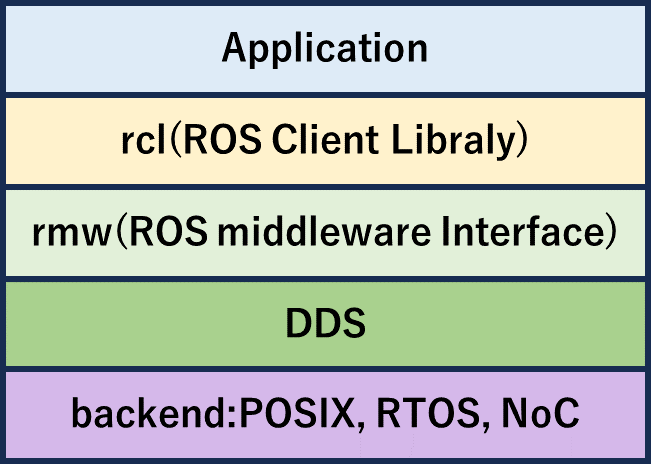
\includegraphics[width=10cm]{images/fig2_ros2_configuration.png}
    \caption{ROS 2の構成図}
    \label{fig:ros2_configuration}
\end{figure}
\begin{figure}[ht]
    \centering
    \begin{minipage}{.48\textwidth}
        \centering
        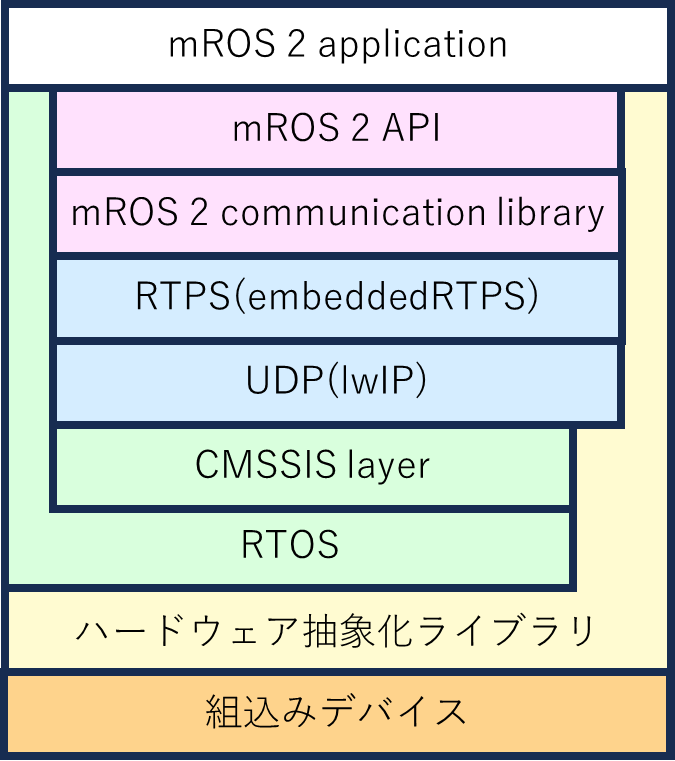
\includegraphics[width=0.9\linewidth]{images/fig1_mros2_b.png}
        \caption{mROS 2の内部構成}
        \label{fig:subfig_a}
    \end{minipage}
    \hfill
    \begin{minipage}{.48\textwidth}
        \centering
        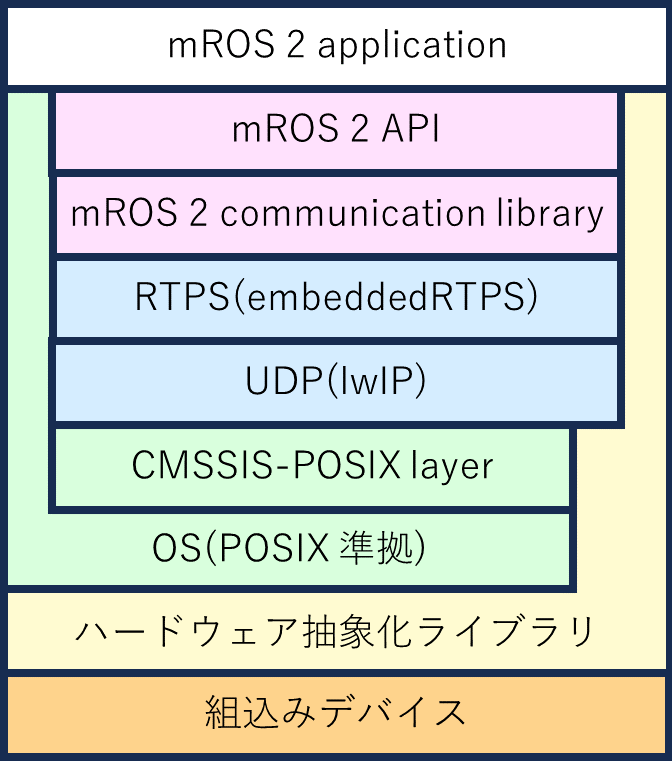
\includegraphics[width=0.9\linewidth]{images/fig1_mros2posix_a.png}
        \caption{mROS 2-POSIXの内部構成}
        \label{fig:subfig_b}
    \end{minipage}
\end{figure}
\begin{table}[ht]
    \caption{QoSの影響}
    \label{tab:qos}
    \centering
    \begin{tabular}{|c|c|c|} \hline
      Publisher & Subscription & 適合性 \\ \hline
      Best effort & Best effort & Yes \\ \hline
      Best effort & Reliable & No \\ \hline
      Reliable & Best effort & Yes \\ \hline
      Reliable & Reliable & Yes \\ \hline
    \end{tabular}
  \end{table}
\section{ROS}
ロボットシステムを開発するにあたって現在はROS 2が主流であるが,その前身であるROSは,スタンフォード人工知能研究所の研究プロジェクトとから移管されたWillow Garage社によって開発が始まったロボットソフトウェア開発基盤である.
最初の正式なディストリビューション版は,2010年3月にリリースされたBox Turtleで,その後,Fuerte,Groovy,Hydro,Indigo,Jade,Kinetic,Lunar,Melodic,Noetic,Foxy,Galactic,Humbleといったバージョンがリリースされている.
ROSの利点は,分散型ロボットシステムの実現に適切である通信ミドルウェアの実装やRTPS(Real Time Publish Subscribe)通信プロトコル,プロジェクト管理やデバックおよびシミュレーションなどのための広範囲なツール群,豊富なOSS(Open Source Software)のパッケージ(ソフトウェアのビルド,実行,共有を容易にするために設計されたフォルダ構造とファイルの集合)やライブラリ(特定の機能やアルゴリズムを実装するプログラムコードの集合),世界規模の活発なオープンソース開発コミュニティという4つの側面にある[8].\\
 まず,通信ミドルウェアの実装やRTPS通信プロトコルによって,開発者が複雑なネットワーク通信の詳細を把握することなく分散型システムの構築に集中できるようになり,リアルタイム性が要求されるアプリケーションの性能を向上させることができる.
\\ 次に,プロジェクト管理やデバックおよびシミュレーションなどのための広範囲なツール群によって,ロボットシステムの開発速度と品質を向上させることができる.
\\ また,豊富なOSSのパッケージやライブラリによって,ロボットシステムの開発速度を加速させ,コストを削減することができる.
\\ 最後に,世界規模の活発なオープンソース開発コミュニティによって,ロボットシステムの開発における技術的な課題を解決するための情報を素早く得ることができる.
これら4つの利点によって,ROSは様々な場所で利用されており,ロボットシステムの開発においては,ROSを利用することが一般的である.
\\ パッケージやライブラリに関しては公式のものだけでも多種多様であり,ロボット本体の制御,モーターの制御,センサーの制御,画像処理,音声認識,自律走行,SLAM(Simultaneous Localization and Mapping)など,ロボットシステムに必要な機能を網羅している.
短期間で機能の大枠を組み立てることができるため,研究開発,教育,産業用途においても,幅広い分野で利用されている.\\
 ROSはすでに10年以上の歴史を持っており,ロボット工学の発展に大きく貢献してきた.
日本の企業ではソニーのaiboの事例がROSを使った製品として代表的であり,他の企業でも商用商品に採用されることも多い.
ロボット開発を取り巻く環境やROSが研究用から商用にも活用され始めるという変遷を受け,2014年より第2世代バージョンであるROS 2の開発が始まった.
これはROS 1が研究用途において,十分な性能を持っていたが,商用製品においてはリアルタイム性やセキュリティの問題があった.
ROS 1の設計は以下のようにされている.
    \begin{itemize}
        \item 単一のロボットで動作することを想定
        \item 多くのリソースを抱えているマシン上で動作されることを想定
        \item リアルタイム性は考慮しない
        \item 優れたネットワーク上で動作されることを想定(有線接続など)
        \item 研究,主に学術的なアプリケーションを想定
        \item 規制や禁止事項がなく,最大限の柔軟性がある(プログラムがmain()から始まることを決定していないなど)
    \end{itemize}
そのため,リアルタイム性を要求する産業用やリソースの少ないマシンに利用されることが増えるとこの設計が問題になることが多かった.
\\ また,ROS 1では利用が広まるにつれて,以下の課題が浮上してきた.
   \begin{enumerate}
       \item メッセージ通信の仲介役としてROS Masterが必要である.ROS Masterが何らかの原因でダウンすると,全てのプロセスがダウンしてしまうという問題がある
       \item リアルタイム性を考慮していない設計になっている
       \item メッセージを暗号化せずに送受信を行っているため,セキュリティに問題がある
       \item 実行するマシンにリソースが少ないと動作が不安定になるという問題がある
       \item Ubuntu(Linux)でないと使いにくい
   \end{enumerate}
そのためROS 2では,上記の問題を解決するため,リアルタイムおよび組込みシステム向けのDDS(Data Distribution Service)[7]と呼ばれる通信ミドルウェアを採用し,通信の信頼性を確保するためのQoS(Quality of Service)制御の機能を導入した.
% QoSは,通信の信頼性や遅延時間,帯域幅などの通信品質を制御するための機能である.
% ROS 2にはQoSの設定として,データの到達を保証するReliability,多少のデータの欠損を許容するBest\_Effortがあり,ROS 2のノードにはデフォルトでReliabilityが設定されている.QoSの説明する
\\ ROSのミドルウェア実装であるDDS[?]の採用により,(1)の問題点がなくなり,QoSとDDSの組み合わせにより,(2)に対してリアルタイム性の実現を目指した.(3)のセキュリティの問題はROS 2でメッセージの暗号化が施されたことにより解決した.また,(4)に対応するためにリソースの少ないマシンで動作できるように開発されている.
さらに,(5)のUbuntu以外のOSにも対応した.
\\ ROS 2の構成を図\ref{fig:ros2_configuration}に示す.
ROS 2ではユーザーが実装するアプリケーション層があり,その下にクライアントライブラリであるrclの層がある.rclクライアントライブラリ層には通信概念を公開するAPIの定義がされており,DDSの上に構築された.rclは,C++,Pythonといった各プログラミング言語用のクライアントライブラリに共通する機能を提供しているAPIである.その下部にrmw(ROS Middleware Interface)とDDSがある.rmwは様々な種類のDDS実装,各backendの差を吸収,最適化を施している層であり,rclクライアントライブラリに対して共通のインタフェースを提供している.DDSはリアルタイム通信を行うためのAPIとプロトコルを提供している国際ミドルウェア標準[24]に基づいて実装された層である.RTPSはDDSから呼び出されるtransport層に位置する通信プロトコルである.backendとして,RTOS(Real Time Operating System)やPOSIXなどのROS 2は様々な環境で動作するためを表す層がある.
\\ 2015年8月には最初のディストリビューションであるアルファ版がリリースされ,2017年の12月にROS 2が本リリースされた.
2023年のMetrics Report[23]によると,ROSは550365601回ダウンロードされている.
そのうち30\%がROSのディストリビューションであるNoeticで,32\%がROS 2のディストリビューションであるhumbleである.
2023年でROSはNoetic,ROS 2はhumbleが主流のディストリビューションであった.
本研究はubuntu 22.04でリリースされたROS 2のhumbleディストリビューションを使用している.
\subsection{PublisherとSubscriber}
ROSでは基本的なノード間のデータ通信としてPublish/Subscribe(Pub/Sub)通信型の非同期な通信プロトコルを採用している.
データの送信側をPublisher(出版者)とよび,受信側をSubscriber(購読者)と呼ぶ.
通信経路として,トピック(Topic)を介した通信が行われる.
トピックで送受信されるデータはメッセージ(Message)と呼ばれ,車輪の角速度や回転量,現在位置の3次元座標など,基本型を組合せた任意の型を定義することができる.
同じ名前のトピックに対して,様々な個数や種類のノードが任意のタイミングで登録,変更,削除ができる.
Publisher側は自由なタイミングでTopicに向けて通信を行い,非同期に動作するSubscriber側は,Publisherからメッセージを受け取った際に対応するコールバック関数が実行される.
\\ ノードはPublisherやSubscriber,またその両方をプログラム次第で変化できるため,ユーザが考えたオリジナルのノードを作成することができる.
この仕様のため,ノード同士の依存が少なくなり,ロボットシステム全体の機能の追加や削除が容易である特性は,柔軟なロボットシステムの構築の一助となる.
% ROS 2でPublisherを作成する際,C++でrclcpp::Nodeクラスの継承からcreate\_publisher(),Pythonでimport rclpy後に.create\_publisher()を行うことでPublisherを作成することができる.
% 同様にSubscriberはC++でrclcpp::Subscriptionクラスを使用してcreate\_subscriber(),Pythonでimport rclpy後にcreate\_subscriberを記述することでSubscriberを作成できる.
\subsection{Service通信とAction通信}
ROS 2では,PublisherとSubscriber以外にもService通信とAction通信がある.
Service通信は,サーバーとクライアントの2つのノード間でリクエストとレスポンスをやり取りする通信である.
これは既存のクライアント・サーバーモデル[15]によく似ており,Subscribeするのではなく,ノードがメッセージの値を欲しいタイミングでリクエストする仕組みになっている.
そのため,ロボットに対する命令やデータの取得,計算結果を受け渡しに適しており,Service通信はリアルタイム性や連続的なデータには向かないが,確実に応答するというロボットシステムにおいて重要な役割を果たす.
さらに,Service通信は同期的な通信であるため,Service通信を行うノードは,Service通信が完了するまで他の処理を行うことができない.
そのため,クライアントの処理を間接的にブロックすることができる.
Service通信はパラメータ設定や取得に使用されることが多い.例として,ロボットの速度やセンサー感度の設定に使用される.他にも,ロボットの状態確認や計算や処理のリクエストなどに用いられる.
\\ 一方,Action通信は,Service通信と同様にサーバーとクライアントの2つのノード間でリクエストとレスポンスをやり取りする通信である.
しかし,Action通信はService通信と異なり,リクエストに対するレスポンスを即座に返すのではなく,リクエストに対するレスポンスを返すまでの間に,進捗状況を返すことができる.
この通信方式によって,長時間のタスクやフィードバックが可能なタスク,中断可能なタスクに適しているため,開発者は柔軟性を保ちながら,ロボットシステムを構築することができる.
長時間のタスクの例として,地図の作成や長距離のナビゲーションなどがある.他にも中断可能なタスクの例として,ロボットが掃除をしている最中に,別のエリアを掃除するよう指示を変更するなどがある.
さらに,Action通信は非同期的な通信であるため,Action通信を行うノードは,Action通信が完了するまで他の処理を行うことができる.
これによって,複雑なタスクを行うノードでもAction通信を用いることで同時に処理することが可能であり,多くのリソースがあるマシンで複数のPublisherやSubscriber,Action,Service通信を抱える高度なノードを動作させることができる.
\subsection{QoS}
 QoSは,通信の信頼性や遅延時間,帯域幅などの通信品質を制御するための機能である.
 ROS 2にはQoSの設定として,データの到達を保証するReliability,多少のデータの欠損を許容するBest\_Effortがあり,ROS 2のノードにはデフォルトでReliabilityが設定されている.
 ノード間の通信において,QoSによる影響を表\ref{tab:qos}に示す.
Best\_EffortのPublisherとBest\_EffortのSubscriberの場合,SubscriberはPublisherからデータを受信できる.
同様にReliableのPublisherとReliableのSubscriberの場合,SubscriberはPublisherからデータを受信できる.
また,PublisherのQoS設定がBest\_Effort,SubscriberのQoS設定がReliableの場合,SubscriberはPublisherからデータを受信できない.
ReliableのPublisherとBest\_EffortのSubscriberの場合,SubscriberはPublisherからデータを受信できる.
このように,SubscriberのQoS設定によって,通信ができるかどうかが変わる.
\section{mROS 2-POSIX}
mROS 2-POSIXとはROS 2の軽量実行環境であるmROS 2をPOSIXに準拠したOSでも使用できることを目的に高瀬らによって作成されたPOSIX対応済みのmROS 2である[6].
mROS 2-POSIXはmROS 2同様,ROS 2を採用するロボットシステムにおいて通信方式とメモリ軽量な実行環境を確立することができる組み込み技術を導入することにより,分散型のロボットシステムにおける応答性やリアルタイム性の向上,消費電力の削減が可能になる.
mROS 2-POSIXに実装されているDDSのembeddedRTPS[17]は組込み向けの軽量なDDSであり,ROS 2のデフォルトのDDSとして利用されているFastRTPS[]と通信ができる.
embeddedRTPSは,Pub/Sub通信の相手と経路を自律的に探索できるように設計され,ROS 2およびRTPSの利点が,組み込み技術導入時に損なわれないようになっている.
\\ mROS 2とmROS 2-POSIXの内部構成の違いを図\ref{fig:subfig_a}と図\ref{fig:subfig_b}に示す.
ユーザーアプリケーションからの階層順で,mROS 2通信ライブラリ,通信プロトコルスタック,RTOS,ハードウェア抽象化ライブラリによって構成される.
mROS 2-POSIX API層および通信ライブラリ層は,メッセージを非同期にPublishやSubscribeするためのコミュニケーションチャネルであるROS 2のTopicに相当するAPIおよび通信機能を提供する階層である.
本階層は,ROS 2のネイティブなクライアント通信ライブラリであるrclcppと互換性を保つように設計されている.
mROS 2通信ライブラリは,ユーザアプリケーションに対して,ROS 2通信のトピックに関する基本的なAPIを提供している.
主なAPIとして void mros2::init(),void mros2::Node::create\_node(),void mros2::Publisher::create\_publisher(),void mros2::Subscriber::create\_subscriber()がある.
利用可能な機能は制限されているものの,組込み技術を導入するROS 2開発者は,汎用OS向けのプログラミングスタイルを踏襲しながらC++によってmROS 2のアプリケーションを実装できる.
その制限として,mROS 2-POSIXはService通信やAction通信には対応していない.
通信プロトコルスタックには,前述のembeddedRTPSを採用している.
UDPについては組込み向けのCによる軽量実装であるlwIP(Light Weight IP)[18]が採用されている.
RTOSには,非常に短い間隔で正確な時間測定を可能にする高分解能タイマ(High Resolution Timer)やシステムが待機状態のときにエネルギー消費を削減できるティックレス(Tickless)の低消費電力な処理遅延機能など,高いリアルタイム性と安全性が求められる軽量な組込みシステムに適した設計がなされている.
\section{WebAssembly}
WebAssembly(Wasm)は,C,C++,C\#,Rustなどの言語で書かれたプログラムをコンパイルのターゲットWeb上でプログラムを高速に実行するために設計された,スタックベースの仮想マシンで実行される仮想命令アーキテクチャである[24][27].
サンドボックスな環境でアプリケーションは実行されるため,ハードウェアや言語,プラットフォームに依存せず,ネイティブに近い実行速度でコードを実行できるという性質がある[24].
Wasmの性質からWebブラウザ以外の実行環境として利用する取り組みがあり,Webの外部でWasmを実行するためのAPI群としてWASI(WebAssembly System Interface)[25]が提案された.
WASIを用いることでファイルやディレクトリ,ネットワークソケットなど,様々なリソースにWasmからアクセスできるようになり,Webブラウザ以外の実行環境として動作するWasmランタイムの開発が進んだ.
\subsection{WAMR}
WebAssemblyの実行環境としてWAMR(WebAssembly Micro Runtime)[26]がある.
WAMR は,組込みやIoT,クラウドなど,様々なプラットフォームで動くようにメモリ消費量が小さくなるよう設計された,オープンソースのWasm ランタイムである.
Wasm プログラムの実行方式としてはWasm バイナリを逐次実行するインタプリタ方式と(Classic),Classicインタプリタを基礎としながらも最適化技術を取り入れ,実行速度を高速にしたFastインタプリタと,事前にWasm バイナリをネイティブバイナリにコンパイルして実行するAoT(Ahead Of Time),Wasm バイナリを実行時にネイティブバイナリにコンパイルして実行するJIT(Just In Time)があり,そのうちAoT とJIT ではネイティブと同等の実行速度で動作する.
また,マルチスレッドやスレッド管理を行うpthread API(POSIX スレッドの標準API)をサポートする組込みライブラリやSocket API をサポートする組込みライブラリも提供されている.
% ROS 2に対応しているDDSの種類として,FastRTPS,RTI Connext DDS,eProsima Micro XRCE-DDSを挙げたが,既存の組込みデバイス向けのROS 2ノード実行環境であるmicro-ROS[16]がある.
% micro-ROSはRTPSの軽量規格であるDDS-XRCE(DDS For Extremely Resource Constrained Enviroments)の実装であるMicro XRCE-DDSを採用している.
% Micro XRCE-DDSは,ホストとしてROS 2ノードを実行するデバイスと通信する際に,Agentノードと呼ばれるノードの稼働が必要となる.
% 通信の仲介の役割をAgentノードは担っており,Agentノードは,ホストデバイス上のROS 2ノードとRTPSに則った通信,組み込みデバイス上のノードとXRCEに則った通信をそれぞれ行うため,
% 応答性とリアルタイム性の低下が懸念される.また,複数の組み込みデバイスを用いる場合,Agent ノードは分散型システム全体の通信を仲介するため,Agentノードの数が増えると通信の遅延が増加する.
% そのためmROS 2は,DDSとしてXRCE-DDSを採用せず,embeddeRTPS[17]を採用している.
% embeddeRTPSは,一つのDomainクラスからParticipant,Writer,Readerの3つのインスタンスが生成される.つまり,初期化処理の段階でembeddedRTPSの提供するPub/Sub通信が利用できるようになる.
% これによってXRCE-DDSのようにAgentノードが必要なく,組み込みデバイス上での通信の遅延を抑えることができる.
% このembeddeRTPSが採用されたのは通信の遅延を抑えることができるだけではない.
% このRTPSは,SPDPとSEDPが実装されており,通信の宛先や受け手として自立性を確保できるRTPSであること点である.
% また,ROS 2で代表的なFastRTPSと通信の確認ができているため親和性が高い点も上げられる.
% 以上の設計思想によりmROS 2は,計算資源の限定的な組み込みデバイス上での稼働を想定した組込みデバイスのリアルタイム性の向上および消費電力の削減ができるソフトウェア基盤である.
% \subsection{mROS 2の内部構成}
% 図2.1にmROS 2の内部構成を示す.
% ユーザーアプリケーションからの階層順で,mROS 2通信ライブラリ,通信プロトコルスタック,RTOS,ハードウェア抽象化ライブラリによって構成される.
% mROS 2通信ライブラリは,ユーザアプリケーションに対して,ROS 2通信のトピックに関する基本的なAPIを提供している.
% 主なAPIとして void mros2::init(),void mros2::Node::create\_node(),void mros2::Publisher::create\_publisher(),void mros2::Subscriber::create\_subscriber()がある.
% 通信プロトコルスタックには,C++で実装されたembeddedRTPSを採用している.先ほど述べたようにこのRTPSにはSPDPとSEDPが実装されており,計算資源の限定的な組込みデバイス上での稼働を想定した設計であるかつ,ROS 2の代表的なRTPSであるFastRTPSと通信の確認できているという理由がある.
% UDPについては組込み向けのCによる軽量実装であるlwIP(Light Weight IP)[18]が採用されている.
% RTOSには,TOPPERS/ASP3カーネル[19]が採用されており,非常に短い間隔で正確な時間測定を可能にする高分解能タイマ(High Resolution Timer)やシステムが待機状態のときにエネルギー消費を削減できるティックレス(Tickless)の低消費電力な処理遅延機能など,高いリアルタイム性と安全性が求められる軽量な組込みシステムに適した設計がなされている.
% lwipはCMSIS-RTOS APIに依存しているため,それぞれのAPI差分を吸収するラッパが用意されている.
% \subsection{mROS 2の通信機能}
% mROS 2の通信機能は,mROS 2の通信ライブラリにあるinit task(初期化処理)とRTPS/UDPと通信ライブラリを介するwrite task(Publish処理)とreader task(Subscribe処理)の3つのタスクに分けられる.
% またアプリケーション層にあるuser task(ユーザーアプリケーション)という開発者が実装するタスクがある.
% user taskは,ROS 2のノードに相当している.Pub/Sub通信を行うアプリケーションである.
% mROS 2のAPIを介してPublishやSubscribeを行うことができる.
% init taskはROS 2としてのノードの情報の初期化を行う.APImros2::init()が呼ばれたときに,対象の組込みデバイスをRTPSのParticipantとして登録する.
% writer taskとreader taskに関しては,PublishおよびSubscribeに関する処理を担う.これらのタスクはuser taskからの依頼をmROS 2APIを介して受け,RTPSの該当機能を立ち上げる.
% writer taskはPublishの依頼を受けて起動し,reader taskはSubscribeの依頼を受けて起動する.
% \subsection{mROS 2-POSIXの内部構成}
% mROS 2がPOSIX[20]に対応したのがmROS 2-POSIXである.
% \\ 図2.2に,mROS 2-POSIXのソフトウェア構成を示す.mROS 2-POSIXアプリケーション層は,ユーザが実装するROS 2ノードに相当する.
% つまり,ROS 2におけるオーバーレイに相当する層である.
% mROS 2-POSIX API層および通信ライブラリ層は,メッセージを非同期にPublishやSubscribeするためのコミュニケーションチャネルであるROS 2のTopicに相当するAPIおよび通信機能を提供する階層である.
% 本階層は,ROS 2のネイティブなクライアント通信ライブラリであるrclcppと互換性を保つように設計されている.
% mROS 2通信ライブラリでは,rclcppのうちpub/sub通信の基本的な機能のみ実装されている.
% 利用可能な機能は制限されているものの,組込み技術を導入するROS 2開発者は,汎用OS向けのプログラミングスタイルを踏襲しながらC++によってmROS 2のアプリケーションを実装できる.
% そのためmROS 2-POSIXはService通信やAction通信には対応していない.
% \\ RTPSプロトコルスタックにはUDPでパブリッシャとサブスクライバC++実装のembeddedRTPSが採用されている.
% UDPについては組込み向けのC実装であるlwIPが採用されている.
% 通信層のembeddedRTPSおよびlwIPはCMSAIS-POSIX[21]に依存しており,図1(b)に示すmROS 2のCMSIS-RTOSを互換した層になっている.
% 最下層にはハードウェアを抽象化したライブラリがある.
% \\ mROS 2-POSIXは図2に示す実行方式を採用している.
% リアルタイムOSでは,組込みマイコンを実行資源の管理対象として,タスク単位でアプリケーションが実行される.
% POSIXにおいてはタスクに相当する概念はプロセスであり,そこから生成されるスレッドを実行単位として処理が進行している.
% しかし,mROS 2-POSIXは実行単位であるノードにPOSIXのスレッドを対応づけ,組込みマイコンでの通信処理におけるイベント割込みについては,POSIX準拠OSにおけるブロッキングAPIの発行に相当させて処理している.
% これらの方式によって,mROS 2-POSIXはPOSIX準拠OS上で仮想ROS 2ノードとして軽量環境下で実行することができる.
% \subsection{オーバーレイとアンダーレイ}
% また,ROS 2には重要な概念にアンダーレイとオーバーレイがある.
% アンダーレイは,完成されたパッケージをインストールするワークスペースであり,安定した環境をオーバーレイに提供するためにある.
% オーバーレイは,ユーザー自身で作成したパッケージを扱うワークスペースであり,先ほどのros2\_wsはオーバーレイにあたる.
% ROS 2ではユーザーが作るノードやパッケージをオーバーレイに作成し,必要に応じてアンダーレイのパッケージを参照して使用するのが一般的である.
% このオーバーレイ上でユーザはcolcon buildを実行し,パッケージをビルドする.
% ユーザーはパッケージをビルドした後,すぐに実行することができない.ROS 2ではsourceコマンドを用いてオーバーレイ環境を読み込むことでアンダーレイがオーバーレイより優先されることなく,開発することができる.
% ROS 2においてオーバーレイとアンダーレイは,複雑化するロボットシステムに柔軟性と拡張性をもたらす概念であることがわかる.
% ROS 2のデバック方法として様々なコマンドが用意されており,ros2 topic listというコマンドを実行することで,現在実行されているトピックの一覧を表示することができる.
% ros2 topic echoは,指定したトピックのメッセージを表示することができる.
% また,現在実行されているノードを視覚的に確認できるようにrqt\_graphと呼ばれるものが用意されている.開発者はrqt\_graphを用いて,目に見えないROS 2のノード間の通信を確認することができる.
% こうしたアンダーレイ機能の充実によって,ROS 2はROS 1よりも柔軟性と拡張性を持つことができた.
% \subsection{ROS 2が対応しているDDS}
% ROS 2の通信ミドルウェアであるDDSと通信プロトコルであるRTPSは,通信相手の探索および通信経路の確立を自律的に行う.
% この機能の実現は,RTPSのSPDP(Simple Participant Discover Protocol)とSEDP(Simple Endpoint Discover Protocol)[9]というプロトコルによって行われる.ここで,RTPSでは,ROS 2のノードに相当するものをParticipant(参加者)と呼ぶ.
% 通信相手を探索するためには自身の情報を送信するモジュールをWriter,ほかのParticipantから情報を受け取るモジュールをReaderと呼ぶ.
% SPDPは,Participantの情報を送受信するためのプロトコルであり,SEDPは,Topicの情報を送受信するためのプロトコルである.
% この通信のエンドポイントは,Participant同士のPublish,Subscribeである.
% \\ RTPSをOSI参照モデルに例えるとtransport層に位置し,UDP/IPの上に実装されている.UDP通信にはパケットの到着に関する保証がないが,ROS 2のDDSではこれを補助するQoS(Quality of Service)制御の機能がある.
% QoS制御は,サブスクライバ,パブリッシャごとに設定でき,厳格な条件であればRELIABLE(信頼性の高い通信)を,緩やかな条件であればBEST EFFORT(ベストエフォート通信)を選択することができる.
% ROS 2のデフォルトDDSであるFastRTPS[10]では,QoS制御の機能が実装されており,各ノードが通信するときのQoS設定はRELIABLEである.
% ROS 2にはデフォルトでFastRTPSというDDSが実装されている.
% DDSとは,OMG(Object Management Group)が定めたデータ交換のための仕様である.これによって分散型ネットワークでも効率的に通信が可能になっている.
% FastRTPSのほかにも,RTI Connext DDS[11]やeProsima Micro XRCE-DDS[12]というDDSがROS 2に対応している.
% Ubuntu22.04のROS 2 humbleでは,FastRTPSはもちろんのこと,デフォルトでEcripse Cyclone DDS[13],Gurum DDS[14],RTI Connext DDSがインストールできる.%リファレンス1[https://docs.ros.org/en/humble/Installation/DDS-Implementations.html#ubuntu-linux-source-install].



% \subsection{mROS 2-POSIXの動作フロー}
% mROS 2-POSIXの動作は以下のようになっている.
% \begin{itemize}
%     \item netif\_posix\_add(NETIF\_IPADDR, NETIF\_NETMASK)によって,lwIPのネットワークインターフェースを初期化する.
%     \item osKernelStart()によって,RTOSのカーネルを起動する.
%     \item mros2::init(0, NULL)によって,mROS 2-POSIXの初期化を行う.
%     \item mros2::Node::create\_node(ノード名)によって,ノードを生成する.
% \end{itemize}
% mROS 2-POSIXは通常のmROS 2と同様にlwipを利用してUDP stackを実装している.
% 異なる点として,mROS 2‐POSIXはPOSIXレイヤが設けられていることが挙げられる.
% このように明確なレイヤを設けたことによって,netif\_posix\_add(NETIF\_IPADDR, NETIF\_NETMASK)のような実装が追加されている.
% 引数に現在mros2-posixをビルドしているマシンのIPアドレスとサブネットマスクを設定することによって,lwIPのネットワークインターフェースを初期化する.
% このNETIF\_IPADDRとNETIF\_NETMASKは,mROS 2-POSIXのヘッダファイルであるmros2\_posix\_netif.hに定義されている.
% そのためビルド前にip aなどで自分のIPアドレスを確認し,そのIPアドレスとサブネットマスクを設定する必要がある.
% この設定をを行わないと,ROS 2やほかのmROS 2ノードと通信できなくなり,ros2 topic listなどのデバックコマンドにも表示されない.
% \\ 次に,osKernelStart()によって,RTOSのカーネルを起動する.その後,mros2::init(0, NULL)によって,mROS 2-POSIXのノードの初期化を行う.
% mros2::init()はmROS 2-POSIXのノードの初期化,つまり,ROS 2としてノード情報を初期化するということである.これは対象の組込みデバイスをRTPSのParticipantとして登録する.
% このタスクを行った後,mros2::init()は休止状態に移行する.
% \\ そして,mros2::Node::create\_node(ノード名)によって,ノードを生成する.この命令に紐づけられたインスタンス変数を介して,Publisherやサブスクライバーを生成する.

% \subsection{mROS 2-POSIXのPublish処理}
% mROS 2-POSIXにおいてPublish処理はmROS 2とほとんど変更がない.
% まず,mros2::Node::create\_publisher()によってmROS 2ノードをPublisherとして登録する.
% mros2::Node::create\_publisherは関数テンプレートとして実装されており,第一引数にトピック名,第二引数にPublishするメッセージのキューのサイズを設定する.
% 例として,mros2::Node::create\_publisher<型名>(トピック名,10)という形で記述する.
% <型>の中に入るのは,Publishするメッセージの型である.ROS 2同様に様々な種類の型を設定でき,ユーザーが自由に定義することができる.
% 同様に"トピック名"にはトピック名が,10はPublishするメッセージのキューサイズ(履歴の長さ)が入る.
% 定義されたpublisherがどのようにPublishされるのか以下にフローを示す.
% \begin{itemize}
%     \item mros2::Publisher.publish()を呼び出す.引数にはメッセージ情報が格納されたオブジェクトのポインタを渡す.
%     \item mROS 2-POSIXの通信ライブラリ内でメッセージのシリアライズを行い,RTPSに則った形式に変換する.
%     \item embeddedRTPSの提供する機能によってUDPパケットを作成し,タスク間通信でmROS 2-POSIXのParticipantのwriterにPublish処理を依頼する
%     \item writerのタスクが実行され,RTPSのSPDPによって,Publisher情報を送信する.
% \end{itemize}
% mROS 2‐POSIXのPublish処理は,mROS 2と同様にUDPパケットを作成し,RTPSのSPDPによって,Publisher情報を送信する.
% mROS 2通信ライブラリの通信処理効率化のためにwriter taskは,CPUとネットワーク通信を平行に行うことができる.
% このため,embeddedRTPSやlwIPにおけるメッセージ,UDPパケットの送信処理に関して,user taskから分離してwriter taskで実行されるようになっている.
% \subsection{mROS 2-POSIXのSubscribe処理}
% mROS 2-POSIXにおいてSubscribe処理もPublish処理と同様にほとんど変わらない.
% mros2::Node::create\_subscription()によってmROS 2ノードをサブスクライバーとして登録し,メッセージをSubscribeできるようにする.
% サブスクリプションも同様に関数テンプレートとして実装されており,テンプレートの仮引数にはメッセージ型,引数にはトピック名とRTPSにおけるQoSのキャッシュに加えて,Subscribe時に呼び出されるコールバック関数を指定する.
% 例として,mros2::Node::create\_subscription<型名>(トピック名,10,コールバック関数)という形で記述する.
% これによってembeddedRTPSに紐づけられたため,Subscribe機能を利用できる.
% 定義されたsubscriberがどのようにSubscribeされるのか以下にフローを示す.
% \begin{itemize}
%     \item ノードのParticipantのreaderがUDPパケットを受信する.
%     \item 初期化タスク時にParticipant情報として登録されていたembeddedRTPS内のコールバック関数が実行され,RTPSに則った形式に変換する
%     \item mROS 2通信ライブラリ内でRTPSパケットのデシリアライズを行い,メッセージに変換する.
%     \item タスク間の通信によって登録されていたコールバック関数およびSubscribeされたメッセージのオブジェクトポインタを渡す.
%     \item メッセージのオブジェクトのポインタを引数としてコールバック関数を実行する.
% \end{itemize}
% メッセージのPub/Sub通信は非同期的に行われるため,reader taskがSubscribeを待ち受けるにはCPU使用権を専有する必要があり,
% メッセージSubscribeに対するコールバック関数を実行する必要がある.その為,この処理時間が長くなる場合に,次のメッセージのSubscribeを待てないという問題が発生する.
% UDPパケットの到着を高い優先度で定期的に監視する役目をreader taskが行うことで到着時にメッセージのSubscribe処理を行うようにしている.
% \subsection{mROS 2-POSIXのメッセージ生成}
% ROS 2では様々なメッセージ型を定義して通信することができるが,mROS 2-POSIXもオリジナルのメッセージファイルを用意してそのメッセージ型で通信することができる.
% そもそもmROS 2にはデフォルトでsensor\_msg/msg/image.hpp,std\_msgs/msg/bool.hpp,byte.hpp,char.hpp,float32.hpp,float64.hpp,header.hpp,int16.hpp,int32.hpp,int64.hpp,int8.hpp,string.hpp,uint16.hpp,uint32.hpp,uint64.hpp,uint8.hppというメッセージ型が用意されている.
% これらのメッセージ型は,mROS 2-POSIXでも利用することができるが,ほかのメッセージ型もmros2/mros2\_header\_generatorの.pyファイルを用いて生成することができる.
% 生成したいメッセージファイルはcustom\_msgs/の中に入れないと生成できない.また階層構造はかならず○○\_msgs/msg/○○.msgという形にしないと生成できない.
% またメッセージファイルのなかにコメント文があるとコメントも一緒に取り込んでsplitするので注意する必要がある.


% chapter 3
\chapter{先行研究}
\begin{figure}[ht]
    \centering
    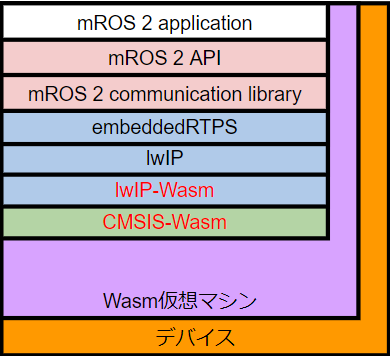
\includegraphics[width=13cm]{images/fig3_mros2-wasm_configuration.png}
    \caption{mROS 2-Wasmの構成図}
    \label{fig:mros2-wasm_configuration}
\end{figure}
\begin{figure}[ht]
    \centering
    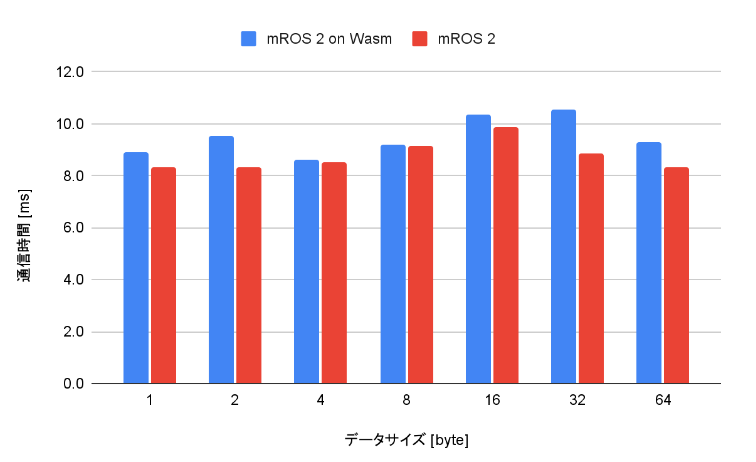
\includegraphics[width=13cm]{images/fig3_kakimoto_pubsubtime.png}
    \caption{mROS 2-Wasmの通信性能}
    \label{fig:mros2-wasm_configuration}
\end{figure}
\begin{figure}[ht]
    \centering
    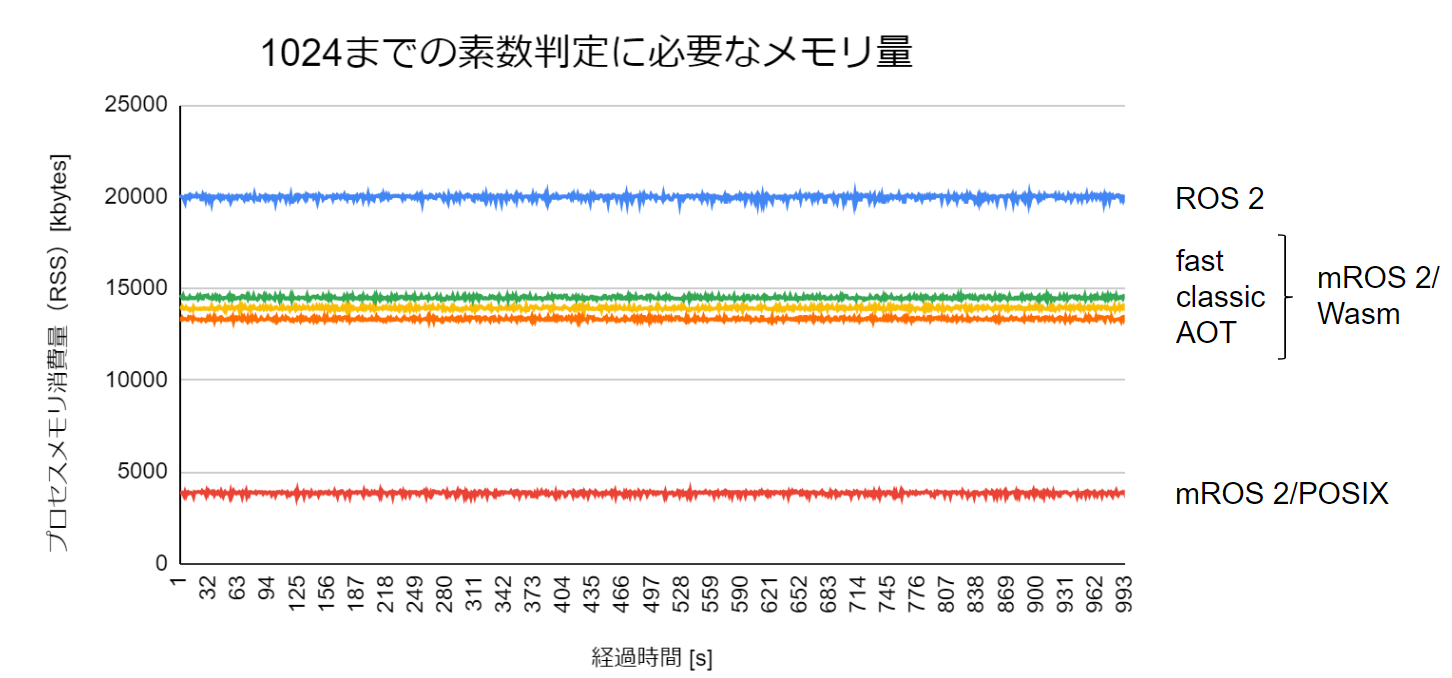
\includegraphics[width=13cm]{images/fig3_mros2-wasm_memory.png}
    \caption{mROS 2-Wasmのメモリ使用量}
    \label{fig:mros2-wasm_configuration}
\end{figure}
柿本らによって,mros2-POSIXをwasm環境で実行するmROS 2-Wasmが提案された.[5]
\\ mROS 2をWasm化させるにともない,使用するWasmランタイムに関して以下の制約がある.
\begin{itemize}
    \item ROSランタイムにはスレッド操作やネットワーク通信の処理が必要であるため,Wasmランタイムにはこれらの機能が必要である
    \item リソースの限られているエッジデバイスで動作させることを想定する必要があるため,WasmランタイムとROSランタイムによるリソース消費を最小限に抑える必要がある
\end{itemize}
Wasmはサンドボックスな環境で実行されるため,OSの機能に依存した層があるmROS 2-POSIXをそのままではコンパイルすることができない.
図2.3で示したとおり,mROS 2-POSIXでOSに依存している層はCMSIS-POSIXとlwIP-POSIXである.
CMSIS-POSIXはmROS 2内部でRTPS通信を行うための機能として,スレッド管理機能,排他制御機能,メッセージキュー管理機能,時間管理機能がpthread(プログラム内で複数の実行スレッドを作成・制御するためのAPIを提供)などを用いて実装されている.lwIPでは,UDPマルチキャストをおこなための実装がSocketやCMSIS-POSIXが提供する機能を用いて実装されている.
\\ これらの依存を解消するため,CMSIS-POSIXをWasm対応したCMSIS-WASM,lwIP-POSIXをWasm対応したlwIP-WASMを柿本らは実装した.
mROS2-wasmの構成を図3.1に示す.
なお,mROS 2はオープンソースソフトウェアであることから上位レイヤに変更が加わっても変更を取り込みやすいよう,既存のビルドシステムに極力手を加えずにシステムを構築されている.
\\ CMSIS-WASMを実装する機能のうち,排他制御機能,メッセージキュー管理機能はスレッド管理機能に依存している.
時間管理機能は手を加えることなくWasmコンパイルが可能であったため,実際に実装されたのはスレッド管理機能である.
実装に際して,WAMRのpthread APIを用いてスレッド管理機能を実装されているがWAMR pthread ライブラリの既知の問題が障害となった.
以下にその問題を述べる.
\begin{itemize}
    \item timespec 構造体をサポートしていない
    \item wasi-sysrootのerrnoと互換性がない
    \item pthread\_attr\_t 構造体をサポートしていない
\end{itemize}
timespec構造体は,スレッドの同期処理などに使われるpthread\_cond\_timedwait 関数から使用され,待機時間の長さを指定するために使われる.WAMRではtimespec構造体が使われず,usecondsを用いる必要があった.そのため待機死体時間をマイクロ秒単位に変換し引数としてWAMRのpthread\_cond\_timewaitに渡すことでtimespec構造体を用いずに同様の動作をさせた.
\\ errnoに関してはシステムが正常に動作している際に使われることがないため,仕様が避けられている.
\\ スレッド生成時にそのスレッドの属性を設定するのに使われるpthread\_attr\_t構造体は,WAMRではサポートされていない.しかし,pthread\_attr\_tはスレッドを生成する関数のみで使用されており,デフォルトの属性から変更されずにスレッド適用されていたため,削除されている.CMSIS-WASMは上記のように柿本らによって実装された.
\\ lwIP-WASMは,Socketを用いて通信機能の実装が行われているため,WASIを用いる必要がある.WAMRにはWASIを用いて実装されたSocket APIが提供されているため,それを用いて実装が行われた.
\\ WAMRのSocket APIでは,setsockopt関数においてIPPROTO\_IPレベルで設定できるオプションは5つに限られている.以下に示すのがそのオプションである.
\begin{itemize}
    \item IP\_MULTICAST\_LOOP
    \item IP\_ADD\_MEMBERSHIP
    \item IP\_DROP\_MEMBERSHIP
    \item IP\_TTL
    \item IP\_MULTICAST\_TTL
\end{itemize}
一方,mROS 2-POSIXのlwIP-POSIXでは,IP\_MULTICAST\_IF,IP\_ADD\_MEMBERSHIP,IP\_MULTICAST\_TTLが使用されており,IP\_MULTICAST\_IFがWAMRのSocket APIには存在しないためネットワークインターフェースの指定ができないという問題があった.SocketはIP\_MULTICAST\_IFによるネットワークインターフェースの指定がない場合はデフォルトのネットワークインターフェースが指定されるため,IP\_MULTICAST\_IFを設定するsetsockopt関数を削除して実装が行われた.また,マルチキャスト通信の配信範囲を制御するTTLを設定するIP\_MULTICAST\_TTLの指定時に,WAMRのSocket APIではオプションデータの長さが4bytesでないときプログラムが終了してしまう.lwIP-POSIXではこの長さが1bytesで定義されていたため4bytesに変更した.このようにWAMRのSocket APIに合わせた細かい変更を行うことで,lwIP-WASMが実装された.
システムのビルドは,外部のプロジェクトのビルド・インストールなどを可能にするExternalProjectを用いてmROS 2のディレクトリ外から行うことができる.
以上の実装により,実行中のmROS 2-POSIXをWasm化することができた.
\\ mROS 2-Wasmは通信時間とメモリサイズと計算処理性能の評価が行われた.
\\ 計算処理性能の評価では,ノード内で擬似作業として1以上の整数を順に素数判定し,1024までの素数を見つける処理を行う実装をし,その時間を計測,評価した.
コンパイル方式はAoTとClassic インタプリタとFast インタプリタを使って計測した.
\\ 通信時間ではmROS 2-WasmとmROS 2を比較評価した.その結果を図3.2に示す.
計測方法はクラウド想定のデバイスから文字列データを送信し,ロボット想定のデバイスからデータを受けとると,そのままデータを返し,クラウド想定のデバイスが受け取るまでの時間,RTT(Round Trip Time)を計測している.mROS 2-Wasmのコンパイル方式はAoTとJITを使わずClassicインタプリタでコンパイルしたバイナリファイルを使って計測した.
\\ メモリサイズの評価では,mROS 2-POSIXとmROS 2-WasmとmROS 2-POSIXを比較評価している.その結果を図3.3に示す.
この計測では,計算処理性能で実装された処理のプロセスIDのRSS(Resident Set Size)とVSS(Virtual Set Size)を取得し評価をした.
今後の課題として,mROS 2-Wasmに実行状態の保存,復元機構を実装することが残った.
%柿本さんの研究の評価方法を載せたい通信性能でAOTとJITは動作しなかったため,Classicでの評価が行われた.ということを言わないといけない
% chapter 4
\chapter{検討手法}
%spheroとraspimouseのwiiboardの手法について話す
%spheroはcgoの話とライブラリ移植の話
%raspimouseは開発環境の話と調査が必要な個所についての話.何と何がうまくいって何がうまくいかなかったのかなど.

\section{Sphero sprk+}
Wii Fit BoardとRaspimouseを用いたロボットの動作を制御するアプリケーションを実装する.
Raspimouseとは,ロボット開発キットであるRaspberry Pi Mouseのことで,Raspberry Pi上で動作するROS 2のノードで制御することができる.
Wii Fit Boardは,任天堂が発売したWiiの周辺機器で,体重移動を検知することができる.
このアプリケーションは,Wii Fit BoardからのセンサデータをRaspimouseにPub-Sub通信を用いて送信し,Raspimouseは受信したセンサデータをもとに動作を制御する.
ユーザの体重移動によってロボットが動作するため,エンドツーエンドのアプリケーションである.
また,Raspimouse上でノードを立ち上げ動作しているため,組み込みデバイス上で動作するアプリケーションという条件も満たしている.
評価実験に用いるアプリケーションとして,Wii Fit BoardとRaspimouseを用いたロボットの動作を制御するアプリケーションを実装するが,本来は,Wii Fit BoardからのセンサデータをSphero sprk +にPub-Sub通信を用いて送信し,Sphero sprk +は受信したセンサデータをもとに動作を制御するアプリケーションを実装する予定だった.
Sphero sprk +は,Sphero社が発売した球体のロボットで,ユーザーがスマートフォンから操作することができる.
ROS 2側ではWii Fit Boardからのセンサデータを受け取り,Sphero sprk +に送信する2つのノードを実装することに成功したが,mROS 2-POSIX側ではWii Fit Boardからセンサデータを送信するノードを完成させることができたものの,Sphero sprk +を受信したセンサデータをもとに動作させるノードの作成が難しく,実装を断念した.
実装を断念した理由として,ROS 2側の実装ではSphero sprk +はPythonのライブラリを用いて制御しており,mROS 2-POSIXはPythonのSupportはないため,動作させるには,PythonのライブラリをC++言語に変換する必要があった.
しかし,PythonのライブラリをC++言語に変換するためには,bluezを用いてSphero sprk +をBLEサーバーと見立てたクライアントのスクリプトを実装する必要があり,その実装が間に合わないと判断したため,実装を断念した.
また,Sphero sprk +を動作させるライブラリはgo言語にもあったため,cgoと呼ばれるgo言語からC言語の関数を呼び出すための仕組みを用いて,go言語からSphero sprk +を動作させることも試みたが,mROS 2-POSIXのcgo移植になってしまい,実装範囲が広くなってしまったため,実装を断念した.
\section{Raspberry Pi Mouse}
実装アプリケーションはROS 2とmROS 2-POSIXの2つの環境で動作する.
ROS 2側のアプリケーションは,C++言語でWii Fit Boardのセンサの値をパブリッシュするノードを実装した.
センサの値をパブリッシュするためには,Wii Fit Boardを端末とBluetooth接続する必要がある.
接続後は/devにある/event○○を開くことでWii Fit Boardのセンサ値を取得できる.しかし,/eventはネットワーク環境によってランダムな/event番号に振り分けられるため,実行するネットワーク環境に変更があるたびに修正しなくてはならない.
また,ノード実行前に/dev/uinputにchmodでa+rwの権限を与えておく必要がある.
Wii Fit Boardはそれぞれの角に4つのセンサがあり,センサの値を/eventから4つの値が取得できる.
この値をこのままパブリッシュすると,サブスクライブする側で4つの値を処理しなくてはならないので,この4つの値をx,yの2つの値に変換する.
x,yはユーザの重心点を表しており,Boardに乗っているユーザの体重に応じてその大きさが変化する.
次に,x,yの値をサブスクライブするノードではパブリッシュされたx,yの値を受け取り,x,yの値に応じてRaspimouseの動作を制御する処理を実装した.
x,yの値はそれぞれユーザの体重によって大きく増減するため,適切な閾値の値はユーザーによって変化する.
今回の場合は,評価実験するユーザーとして開発者のみになるため,開発者の体重に合わせた閾値の値を設定した.
ロボットが動作する処理は,x,yの値が閾値を超えた場合にRaspimouseが動作するように実装した.
ユーザーがロボットを前進させようとした時,yの値がマイナスに大きく傾くため,yの値がマイナスの閾値を超えた場合にRaspimouseが前進するように実装した.
同様に,yの値がプラスに傾くとき,ロボットを後退させ,xの値がマイナスに傾くときにロボットを右に移動させ,プラスに傾くときにロボットを左に移動させるように実装を行った.
ロボットを移動させる処理はロボットのデバイスドライバを直接write命令を用いてたたくことで実装を行っている.
mROS 2-POSIX側のアプリケーションは,ROS 2側のアプリケーションと大きく変更されていない.
ROS 2側のアプリケーションと同様にWii Fit Boardのセンサの値をパブリッシュするノードを実装し,その値をサブスクライブするノードを実装した.
パブリッシュするノードではROS 2側と同様の実装になっている.異なる点はROS 2側ではrclcppと呼ばれるROS 2のノードを作成するためのインターフェースを使用しているが,mROS 2ではオリジナルのインターフェースが用意されている.
\subsection{実装に際しての課題}
実装に際しての課題としてWii Fit Boardの値をパブリッシュするノードとその値をサブスクライブし,Raspimouseを動作させるノードそれぞれであった.
Wii Fit Boardの値をパブリッシュするノードでは,mROS 2-POSIX側のノードで実行後にSegment Faultが発生した.
mROS 2-POSIXを利用していると,ビルドが通って実行時にPub-Sub通信の準備が完了した後,Segment Faultが発生することがある.
これによって,ノードが突然動作しなくなる問題があったが,再度ビルドすることで修正することができた.
Wii Fit Boardのセンサの値をパブリッシュするノードからサブスクライブするノードでは,Raspimouseを動作させる部分で課題があった.
Raspimouseを制御する方法としてROS 2を利用する方法が一般的である.方法としては,Raspimouseの制御ノードを立ち上げ,制御ノードがパブリッシュしているトピックを別のノードでサブスクライブしたり,制御ノードがサブスクライブしているトピック宛に値をパブリッシュすることでRaspimouseを操作する.
すでにキーボードやゲームコントローラを使ってRaspimouseを操作できるノードも配布されている.
このRaspimouseの操作だがROS 2側では操作できるノードが配布されているため,比較的容易に動作させることができた.
しかし,mROS 2-POSIX側でRaspimouseの制御ノードであるROS 2のトピックに対してパブリッシュを動作させることができなかった.制御ノードがパブリッシュしている値のサブスクライブは問題なくmROS 2-POSIX側で可能であった.
制御ノードに対してmROS 2-POSIXからのパブリッシュが通らない理由として,QoS設定の問題がある.

% chapter 5
\chapter{実装}
%ラズパイマウスのfollowerノードについての実装を書く.今はspheroとラズパイマウスのwiibordを本実装として話しているため改変が必要。aproachに持っていく。
\label{chap:implementation}
本章では,mROS 2-POSIXとROS 2の性能を比較評価するにあたって,mROS 2-POSIXとROS 2に実装するアプリケーションの概要と,これまで実装予定だったものについて説明する.
\section{実装アプリケーションの概要}
\label{chap:evaluation}章で述べたように,実装するアプリケーションの条件として,Pub-Sub通信のみを使用したアプリケーションであること,組み込みデバイス上で動作できるアプリケーションであること,エンドツーエンドのアプリケーションであることを設けた.
これらの条件を満たすアプリケーションとして,Wii Fit BoardとRaspimouseを用いたロボットの動作を制御するアプリケーションを実装する.
Raspimouseとは,ロボット開発キットであるRaspberry Pi Mouseのことで,Raspberry Pi上で動作するROS 2のノードで制御することができる.
Wii Fit Boardは,任天堂が発売したWiiの周辺機器で,体重移動を検知することができる.
このアプリケーションは,Wii Fit BoardからのセンサデータをRaspimouseにPub-Sub通信を用いて送信し,Raspimouseは受信したセンサデータをもとに動作を制御する.
ユーザの体重移動によってロボットが動作するため,エンドツーエンドのアプリケーションである.
また,Raspimouse上でノードを立ち上げ動作しているため,組み込みデバイス上で動作するアプリケーションという条件も満たしている.
\section{実装予定だったアプリケーション}
評価実験に用いるアプリケーションとして,Wii Fit BoardとRaspimouseを用いたロボットの動作を制御するアプリケーションを実装するが,本来は,Wii Fit BoardからのセンサデータをSphero sprk +にPub-Sub通信を用いて送信し,Sphero sprk +は受信したセンサデータをもとに動作を制御するアプリケーションを実装する予定だった.
Sphero sprk +は,Sphero社が発売した球体のロボットで,ユーザーがスマートフォンから操作することができる.
ROS 2側ではWii Fit Boardからのセンサデータを受け取り,Sphero sprk +に送信する2つのノードを実装することに成功したが,mROS 2-POSIX側ではWii Fit Boardからセンサデータを送信するノードを完成させることができたものの,Sphero sprk +を受信したセンサデータをもとに動作させるノードの作成が難しく,実装を断念した.
実装を断念した理由として,ROS 2側の実装ではSphero sprk +はPythonのライブラリを用いて制御しており,mROS 2-POSIXはPythonのSupportはないため,動作させるには,PythonのライブラリをC++言語に変換する必要があった.
しかし,PythonのライブラリをC++言語に変換するためには,bluezを用いてSphero sprk +をBLEサーバーと見立てたクライアントのスクリプトを実装する必要があり,その実装が間に合わないと判断したため,実装を断念した.
また,Sphero sprk +を動作させるライブラリはgo言語にもあったため,cgoと呼ばれるgo言語からC言語の関数を呼び出すための仕組みを用いて,go言語からSphero sprk +を動作させることも試みたが,mROS 2-POSIXのcgo移植になってしまい,実装範囲が広くなってしまったため,実装を断念した.
\section{実装アプリケーションの詳細}
実装アプリケーションはROS 2とmROS 2-POSIXの2つの環境で動作する.
ROS 2側のアプリケーションは,C++言語でWii Fit Boardのセンサの値をパブリッシュするノードを実装した.
センサの値をパブリッシュするためには,Wii Fit Boardを端末とBluetooth接続する必要がある.
接続後は/devにある/event○○を開くことでWii Fit Boardのセンサ値を取得できる.しかし,/eventはネットワーク環境によってランダムな/event番号に振り分けられるため,実行するネットワーク環境に変更があるたびに修正しなくてはならない.
また,ノード実行前に/dev/uinputにchmodでa+rwの権限を与えておく必要がある.
Wii Fit Boardはそれぞれの角に4つのセンサがあり,センサの値を/eventから4つの値が取得できる.
この値をこのままパブリッシュすると,サブスクライブする側で4つの値を処理しなくてはならないので,この4つの値をx,yの2つの値に変換する.
x,yはユーザの重心点を表しており,Boardに乗っているユーザの体重に応じてその大きさが変化する.
次に,x,yの値をサブスクライブするノードではパブリッシュされたx,yの値を受け取り,x,yの値に応じてRaspimouseの動作を制御する処理を実装した.
x,yの値はそれぞれユーザの体重によって大きく増減するため,適切な閾値の値はユーザーによって変化する.
今回の場合は,評価実験するユーザーとして開発者のみになるため,開発者の体重に合わせた閾値の値を設定した.
ロボットが動作する処理は,x,yの値が閾値を超えた場合にRaspimouseが動作するように実装した.
ユーザーがロボットを前進させようとした時,yの値がマイナスに大きく傾くため,yの値がマイナスの閾値を超えた場合にRaspimouseが前進するように実装した.
同様に,yの値がプラスに傾くとき,ロボットを後退させ,xの値がマイナスに傾くときにロボットを右に移動させ,プラスに傾くときにロボットを左に移動させるように実装を行った.
ロボットを移動させる処理はロボットのデバイスドライバを直接write命令を用いてたたくことで実装を行っている.
mROS 2-POSIX側のアプリケーションは,ROS 2側のアプリケーションと大きく変更されていない.
ROS 2側のアプリケーションと同様にWii Fit Boardのセンサの値をパブリッシュするノードを実装し,その値をサブスクライブするノードを実装した.
パブリッシュするノードではROS 2側と同様の実装になっている.異なる点はROS 2側ではrclcppと呼ばれるROS 2のノードを作成するためのインターフェースを使用しているが,mROS 2ではオリジナルのインターフェースが用意されている.
\section{実装に際しての課題と解決方法}
実装に際しての課題としてWii Fit Boardの値をパブリッシュするノードとその値をサブスクライブし,Raspimouseを動作させるノードそれぞれであった.
Wii Fit Boardの値をパブリッシュするノードでは,mROS 2-POSIX側のノードで実行後にSegment Faultが発生した.
mROS 2-POSIXを利用していると,ビルドが通って実行時にPub-Sub通信の準備が完了した後,Segment Faultが発生することがある.
これによって,ノードが突然動作しなくなる問題があったが,再度ビルドすることで修正することができた.
Wii Fit Boardのセンサの値をパブリッシュするノードからサブスクライブするノードでは,Raspimouseを動作させる部分で課題があった.
Raspimouseを制御する方法としてROS 2を利用する方法が一般的である.方法としては,Raspimouseの制御ノードを立ち上げ,制御ノードがパブリッシュしているトピックを別のノードでサブスクライブしたり,制御ノードがサブスクライブしているトピック宛に値をパブリッシュすることでRaspimouseを操作する.
すでにキーボードやゲームコントローラを使ってRaspimouseを操作できるノードも配布されている.
このRaspimouseの操作だがROS 2側では操作できるノードが配布されているため,比較的容易に動作させることができた.
しかし,mROS 2-POSIX側でRaspimouseの制御ノードであるROS 2のトピックに対してパブリッシュを動作させることができなかった.制御ノードがパブリッシュしている値のサブスクライブは問題なくmROS 2-POSIX側で可能であった.
制御ノードに対してmROS 2-POSIXからのパブリッシュが通らない理由として,QoS設定の問題がある.

\section{実装アプリケーション変更に伴って生じる影響}



% chapter 6
\chapter{実験}
%評価基準として話を変えないといけない.どちらかというと
\label{chap:evaluation}
\begin{table}[ht]
  \caption{実験環境}
  \label{tab:experiment}
  \centering
  \begin{tabular}{|c|c|} \hline
    ハードウェア & Raspberry Pi 3B+ \\ \hline
    OS & Ubuntu 22.04 LTS \\ \hline
    CPU & 1.4GHz 64-bit quad-core ARM Cortex-A53 \\ \hline
    メモリ & 1GB LPDDR2 SDRAM \\ \hline
    ROS 2 & ROS 2 humble \\ \hline
  \end{tabular}
\end{table}

\begin{table}[ht]
  \centering
  \begin{tabular}{|l|c|c|c|}
  \hline
  /light\_sensors & ROS2 & mROS2 & mROS2-Wasm \\ \hline
  平均値 & 733.40μs & 656.59μs & 2101.89μs \\ \hline
  最大値 & 830μs & 780μs & 2870μs \\ \hline
  最小値 & 650μs & 580μs & 1740μs \\ \hline
  標準偏差 & 58.14μs & 51.16μs & 282.89μs \\ \hline
  \end{tabular}
  \caption{/light\_sensorsの通信時間の統計}
  \label{tab:light_sensors_stats}
\end{table}

\begin{table}[ht]
  \centering
  \begin{tabular}{|l|c|c|c|}
  \hline
  /cmd\_vel & ROS2 & mROS2-POSIX & mROS2-Wasm \\ \hline
  平均値 & 42757.34μs & 36954.83μs & 46760.56μs \\ \hline
  最大値 & 74220μs & 72490μs & 83190μs \\ \hline
  最小値 & 16550μs & 2380μs & 14170μs \\ \hline
  標準偏差 & 23451.16μs & 20486.34μs & 20424.32μs \\ \hline
  \end{tabular}
  \caption{/cmd\_velの通信時間の統計}
  \label{tab:cmd_vel_stats}
\end{table}

\begin{table}[ht]
  \centering
  \begin{tabular}{|l|c|c|c|}
  \hline
   & ROS2 & mROS2-POSIX & mROS2-Wasm \\ \hline
  RES(Resident Size) & 32.51MB & 1.66MB & 17.37MB \\ \hline
  SHR(Shared Memory) & 25.16MB & 1.48MB & 1,73MB \\ \hline
  RSS(Resident Set Size) & 57.67MB & 3.14MB & 19.10MB \\ \hline
  \end{tabular}
  \caption{各環境の物理消費メモリ(RSS)}
  \label{tab:rss_stats}
\end{table}

\begin{figure}[ht]
  \centering
  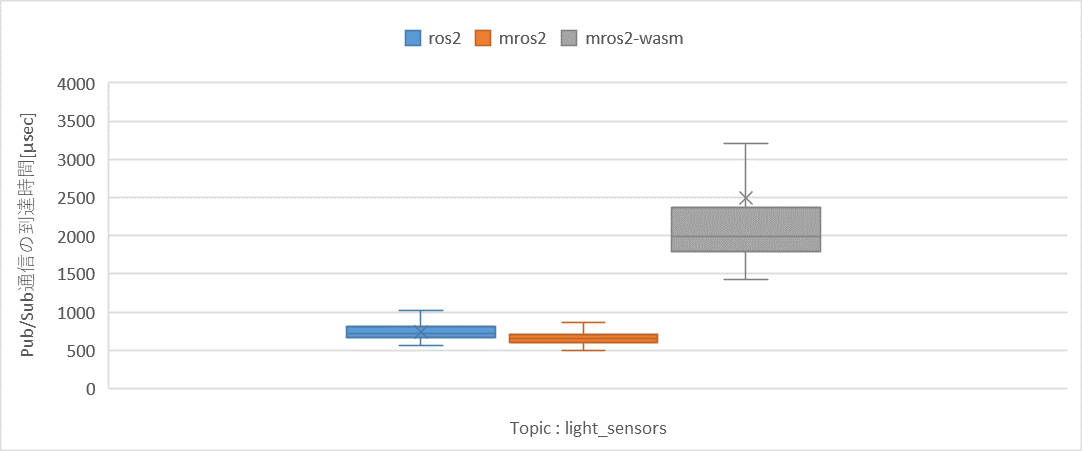
\includegraphics[width=15cm]{images/fig6_lightsensors.png}
  \caption{トピック: /light\_sensorsの通信時間の箱ひげ図}
  \label{fig:light_sensors}
\end{figure}
\begin{figure}[ht]
  \centering
  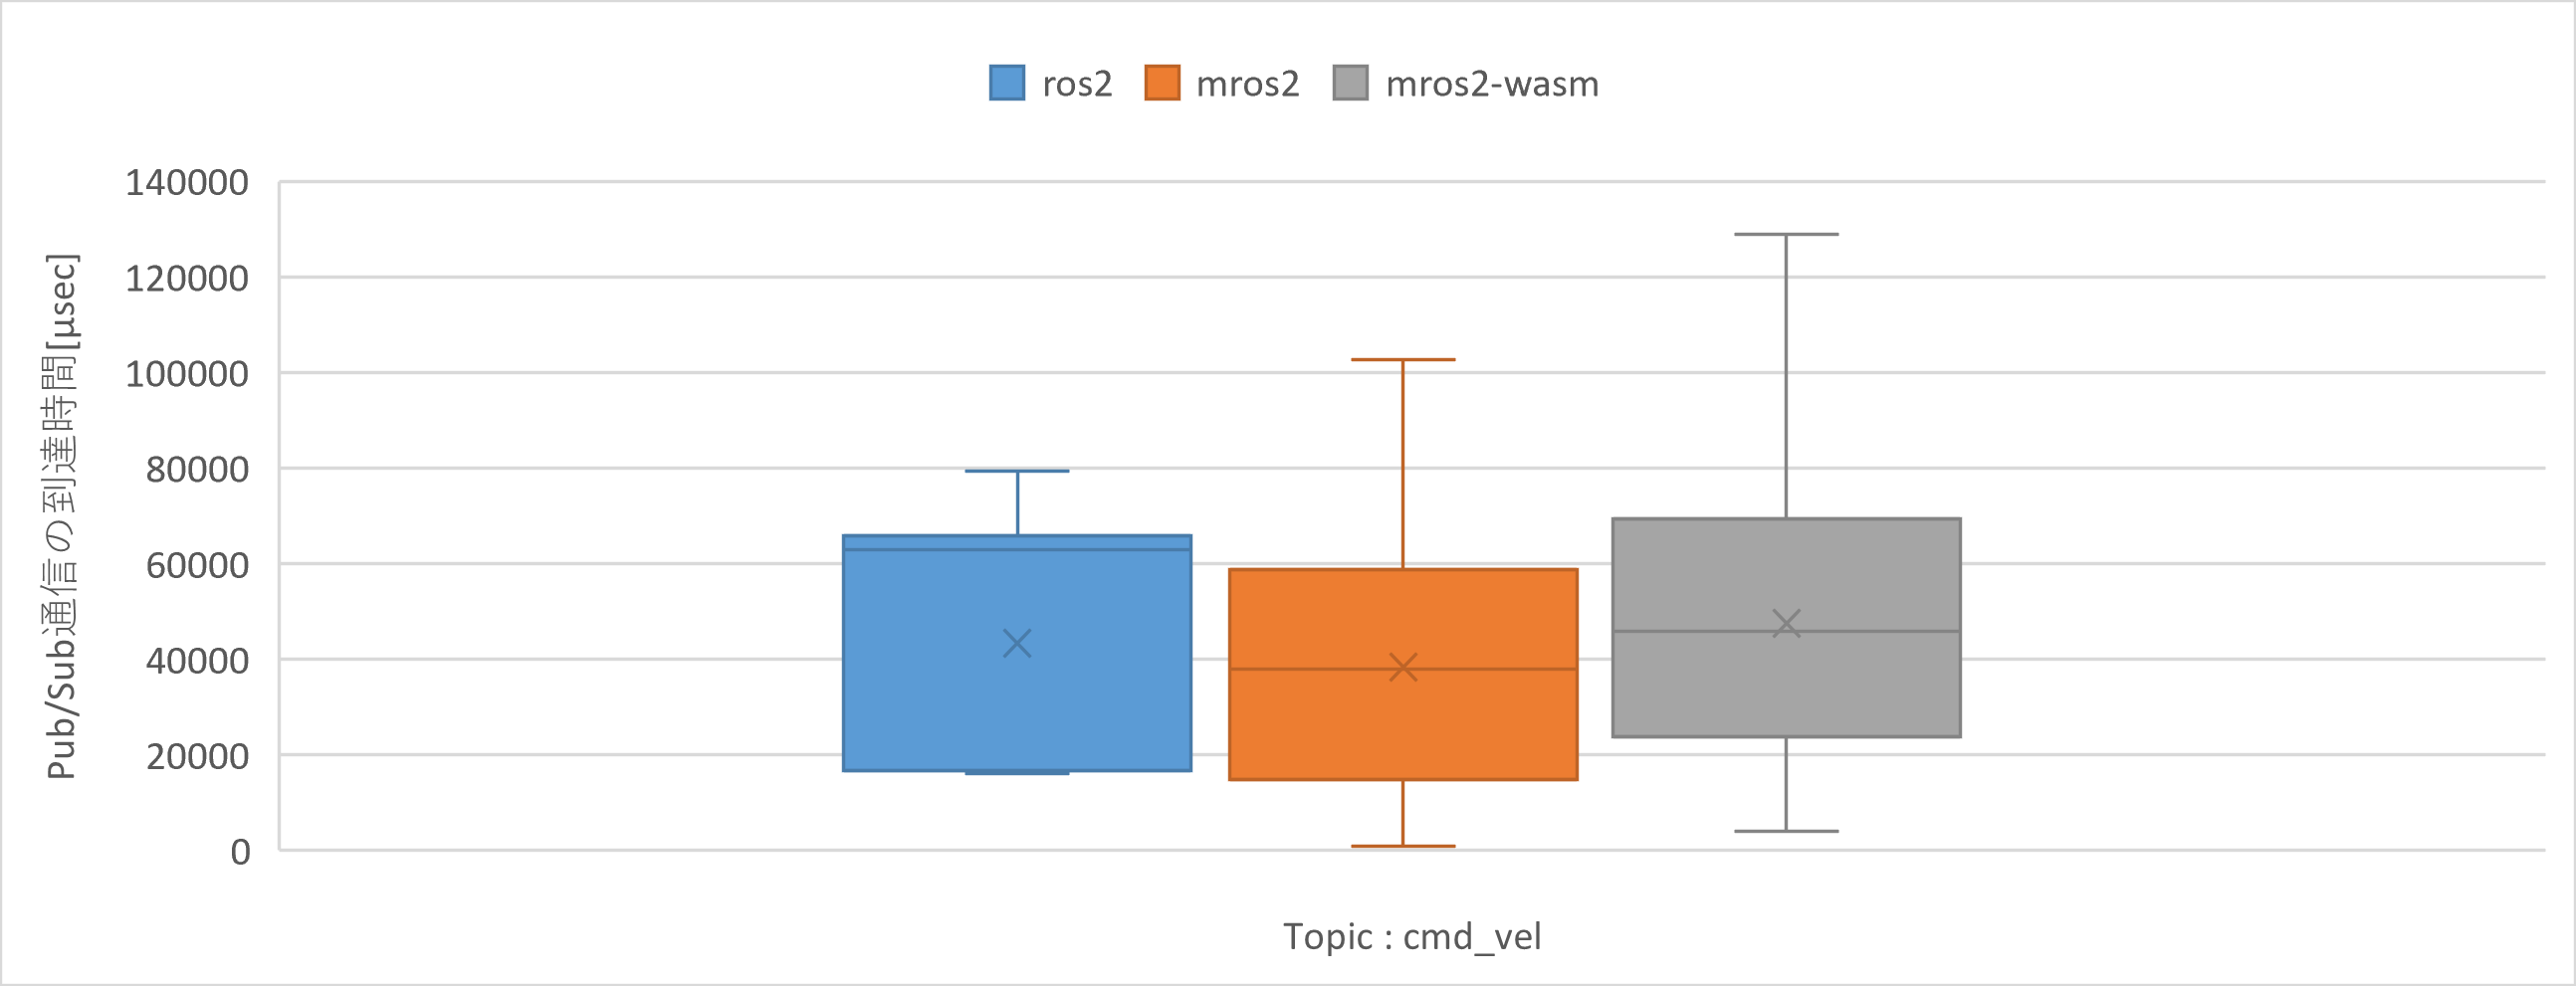
\includegraphics[width=15cm]{images/fig6_cmdvel.png}
  \caption{トピック: /cmd\_velの通信時間の箱ひげ図}
  \label{fig:cmd_vel}
\end{figure}
\begin{figure}[ht]
  \centering
  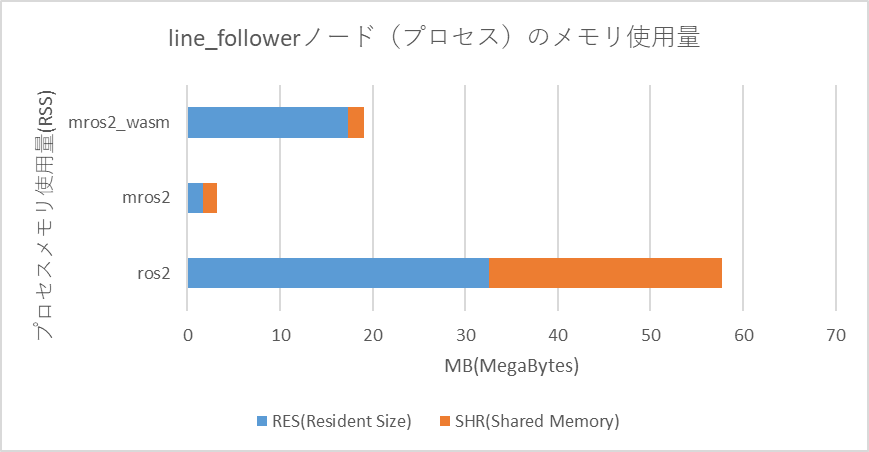
\includegraphics[width=15cm]{images/fig6_memory_v2.png}
  \caption{各環境でRES,SHRを合わせたRSSの比較}
  \label{fig:allmemory}
\end{figure}
本章では,実装したアプリケーションを用いて,mROS 2-POSIXとmROS 2-WasmとROS 2の性能を比較評価した実験について述べる.
\section{概要}
本研究でmROS 2-POSIX,mROS 2-Wasm,ROS 2の性能を比較評価するために,それぞれの環境に実装したライントレースノードをラズパイマウスにジョイントしているRassberry Pi 3B +上で動作させ,制御ノードとライントレースノードの通信時間とメモリ消費量を比較する実験を実施した.
この評価の目的は,ROS 2とmROS 2-POSIX,mROS 2-Wasmの通信性能とメモリ消費量を実アプリケーション上の値をもとに比較し,実アプリケーション上でもmROS 2-POSIXが動的配置機構のソフトウェア基盤として適しているか,そして,mROS 2-Wasmを実アプリケーション上で動作させた場合でも,mROS 2-POSIXの軽量という利点を損なわないかを示すことである.
\\ 実験の実行環境を表\ref{tab:experiment}に示す.なお,第2章で述べた通り,ネイティブROS 2のランタイムディストリビューションは最新版であるhumbleを採用した.
\\ 通信時間の計測は,2つのノード間でPub/Sub通信にかかる時間をLinux標準のclock\_gettime()を用いた.
clock\_gettime()といっても,様々な実装があり,実時間を計測するシステム全体で一意な時間を取得するCLOCK\_REALTIMEや,ある開始地点からの単調増加の時間で表現されるCLOCK\_MONOTONICなどがある.
今回計測に用いたのはCLOCK\_MONOTONICである.
これは,
時間を計測するトピックは,/light\_sensorsと/cmd\_velである.
このトピックはライントレースする際に使用する主なトピックであり,第4章で述べた通り,/light\_sensorsはライトセンサの値を,/cmd\_velはラズパイマウスのモーターを制御するためのトピックである.
/light\_sensorsはInt16型が4つ格納されている配列であり,/cmd\_velはgeometry\_msgs/Twist型で,float64型が6つ格納されている配列である.
この2つのトピックのPublishした現在時刻,Subscribeした現在時刻を取得し,その差分を通信時間とした.
評価にあたって,試行回数を1000回とし,平均値,最大値,最小値,標準偏差を計算し,通信時間の箱ひげ図を作成した.
/light\_sensorsと/cmd\_velのPub/Subの関係は第5章で述べた通り,/light\_sensorsは制御ノードからPublishされるトピックであり,mROS 2-POSIX,mROS 2-WasmはSubscribeするトピックである.
/cmd\_velはmROS 2-POSIX,mROS 2-WasmがPublishするトピックであり,制御ノードがSubscribeするトピックである.
\\ メモリ消費量の計測は,mROS 2-POSIX,mROS 2-Wasm,ROS 2の各環境でのライントレースノードに対して,実行しているランタイムのプロセスIDを取得し,そのプロセスに割り当てられているRSS(物理消費メモリ)を計測した.
各環境で同様の計測を行い,RSSは時間によって変化しなかったため,このRSSを用いて,グラフを作成した.
\section{結果}
実験結果を図\ref{fig:light_sensors}から図\ref{fig:allmemory}および表\ref{tab:light_sensors_stats}から表\ref{tab:rss_stats}に示す.
\\ 図\ref{fig:light_sensors}では各環境ごとにトピック/light\_sensorsのPublishした現在時刻とSubscribeした現在時間の差を計算し,箱ひげ図として通信時間のばらつきを示している.
ROS 2とmROS 2-POSIXの通信時間のばらつきは比較的同等であるが,mROS 2-Wasmを見ると,非常に大きなばらつきがあった.
\\ 表\ref{tab:light_sensors_stats}は,トピック/light\_sensorsに対して各環境ごとに通信時間の平均値,最大値,最小値,標準偏差を示している.
表\ref{tab:light_sensors_stats}を見ると,一番小さい平均値を記録したのがmROS 2-POSIXであり,次いでROS 2,mROS 2-Wasmの順である.
mROS 2-POSIXとROS 2の平均時間の差は約77μsecであり,mROS 2-POSIXとROS 2の通信時間の平均がおおよそ同程度,またはmROS 2-POSIXのPub/Sub通信の方がROS 2よりも若干高速であることだった.
標準偏差は測定値の分布が平均値のまわりにどの程度集まっているか示す指標で小さい順に,mROS 2-POSIX,ROS 2,mROS 2-Wasmの順である.
mROS 2-POSIXとROS 2の差はほとんどなく,若干ROS 2のばらつきが大きいが,ほとんど同程度であった.
mROS 2-Wasmの通信時間の平均がmROS 2-POSIXとROS 2はおおよそ同等であることのに比べて,およそ3倍になっており,標準偏差は,mROS 2-POSIXとROS 2がおおよそ同等であるのに対し,mROS 2-Wasmはおよそ5倍の値になっている.
\\ 図\ref{fig:cmd_vel}は,図\ref{fig:light_sensors}と同様に各環境ごとの/cmd\_velの通信時間のばらつきを示す箱ひげ図である.
図\ref{fig:cmd_vel}を見ると,mROS 2-POSIXとROS 2とmROS 2-Wasmの通信時間のばらつきはほぼ同等であった.
\\ 表\ref{tab:cmd_vel_stats}は,表\ref{tab:light_sensors_stats}同様トピックの/cmd\_velの通信時間の平均値,最大値,最小値,標準偏差を示している.
表\ref{tab:cmd_vel_stats}の平均値は,小さい順にmROS 2-POSIX,ROS 2,mROS 2-Wasmの順である.
mROS 2-POSIXとROS 2の差は5082μsecであり,mROS 2-POSIXの方が遅延が少なかった.
また,ROS 2とmROS 2-Wasmの差は4003μsecであり,ROS 2の方が遅延が少なかった.
標準偏差を見ると,小さい順にmROS 2-Wasm,mROS 2-POSIX,ROS 2の順である.
これは平均値の順と逆であり,mROS 2-WasmとmROS 2-POSIXの差はほとんどなく,ROS 2の標準偏差はmROS 2-WasmとmROS 2-POSIXで大きくことなっている.
\\ 図\ref{fig:allmemory}は,ライントレースノードを各環境で動作させたときのRES(Resident Size),SHR(Shared Memory)を合わせたRSSの棒グラフである.
表\ref{tab:rss_stats}は,各環境のRES,SHR,RSSをそれぞれ数字で示している.
図\ref{fig:allmemory},表\ref{tab:rss_stats}を見ると,mROS 2-POSIXのメモリ消費量がもっとも小さく,次いでmROS 2-Wasm,ROS 2の順である.
mROS 2-POSIXはROS 2やmROS 2-Wasmと比べて非常に小さなメモリ消費量であった.
ROS 2との差は54.53MBである.
mROS 2-WasmはROS 2よりもメモリ消費量が38.57MBと少なく,mROS 2-POSIXのほうが15.96MB少ない.
\section{考察}
図\ref{fig:light_sensors},表\ref{light_sensors_stats},図\ref{fig:cmd_vel},表\ref{tab:cmd_vel_stats}から,mROS 2-POSIXはROS 2と比べてPub/Sub通信の遅延が少なく,安定かつ高速に通信できていることが分かった.
これは,mROS 2-POSIXが組込み用デバイス向けであるDDSのembeddedRTPSが軽量なTCP/IPスタックであるlwIPを採用しているためだと考える.
そして,ROS 2とmROS 2-Wasmの通信時間を比べると,ROS 2側がSubscribeを行い,mROS 2-Wasm側がPublishを行うトピック/cmd\_velでは平均の遅延の差は約4000μsec,mROS 2-Wasmの遅延が大きかったものの,標準偏差はROS 2よりも小さかった.
mROS 2-WasmがROS 2からPublishされたメッセージをSubscribeしているトピック/light\_sensorsでは,mROS 2-Wasmの遅延がROS 2の時よりも平均で3倍ほど大きく,標準偏差はおよそ5倍になっていた.
これは,mROS 2-WasmがClassicインタプリタでコンパイルされ実行されているのが原因であると考える.
しかし,Classicインタプリタで実行されたノードでもPublishの通信時間はROS 2とそこまで大きな差がないということが示された.
この原因として,Publisherの実装がコールバック関数を呼び出す必要のあるSubscriberと比べて,メッセージ処理に時間がかかってしまい,遅延が大きくなると考える.
\\ 通信性能の評価では,実アプリケーション上でmROS 2-POSIXはROS 2よりも高速で動作することが示された.
また,mROS 2-WasmはClassicインタプリタでコンパイルされた場合,遅延がほかの環境よりも大きくなることが示された.
\\ 図\ref{fig:allmemory}と表\ref{tab:rss_stats}から,mROS 2-POSIXはROS 2と比べてメモリ消費量が少ないということがわかった.
これはmROS 2-POSIXがROS 2で実装されているアプリケーションでも軽量なランタイムとして機能しているということを示している.
mROS 2-WasmはROS 2と比べてメモリ消費量が少なく,mROS 2-POSIXと比べてメモリ消費量が大きいということがわかった.
これは,mROS 2-WasmはmROS 2-POSIXをWasm化したものであり,Wasm分のメモリ消費がmROS 2-POSIXに計上されているため,mROS 2-POSIXよりもメモリ消費量が大きいからである.
ネイティブのROS 2よりもメモリ消費量が少ないことで,ROS 2を動作させるよりも,mROS 2-Wasmを動作させたほうがメモリ消費量の削減が可能であることが示された.
\\ 今回の実験によって,実アプリケーションを動作させても,mROS 2-POSIXはROS 2よりメモリ消費量と通信性能で優れており,リソースの限られたデバイスでノードを実行する場合,mROS 2-POSIXのほうがROS 2よりも適していることを示すことができた.
mROS 2-POSIXをWasm化したmROS 2-Wasmは実アプリケーションをClassicインタプリタでコンパイルした場合,通信性能でROS 2よりも劣るものの,メモリ消費量でROS 2より優れていることから,ROS 2をWasm化するよりmROS 2-POSIXをWasm化することでメモリ使用量の削減ができることを示せた.
ただ,通信性能の劣化はコンパイル方式をJITもしくはAOTにすることで改善することができる可能性がある.
先行研究でソフトウェア基盤として採用されたmROS 2-POSIXは実アプリケーション上でも軽量ソフトウェア基盤として最適であり,mROS 2-Wasmを実アプリケーション上で動作させた場合でも,mROS 2-POSIXの軽量という利点を損なわずWasm化することができていることを示した.


% chapter 7
\chapter{関連研究}
%関連研究としては高瀬先生の話とsoraさんの評価実験の話をする.soraさんの話はround tripの参考にしたなど.
この章では本研究の関連研究について述べる.
\section{mROS 2:組込みデバイス向けのROS 2ノード軽量実行環境}
組込みデバイス向けの高効率なROS 2通信方式およびメモリ軽量な実行環境を確立するために,
高瀬らは提案として軽量ランタイムであるmROS 2を設計,実装,評価した.mROS 2を評価するにあたって,
ROSとmicro-ROSを用いている.micro-ROSはROS 2の組込みデバイス向けの軽量実行環境である.
mROS 2とmicro-ROSの違いは,ROS 2と通信する際のAgentノードの有無である.Agentノードを立ち上げなければならない,micro-ROS は通信に遅延が発生する恐れがある.
通信性能の評価実験としてstd\_msgs::msg::Int32のメッセージをエコーバックするアプリケーションを用いている.
アプリケーションでのRTT(Round Trip Time)を計測することで通信性能を評価した.結果は,mROS 2のRTTが一番小さくなり次いで汎用デバイス同士をつないだROS 2環境が速かった.
メモリサイズの比較では,mROS 2がROS 2よりもメモリ消費量が少なかった.
この実験結果から組込みデバイス上で動作したmROS 2のRTTは汎用デバイス上で動作したROSよりも高速であることが分かった.
この評価手法のメモリサイズ消費量について本研究で参考にした.
しかし,通信性能の評価手法は本研究では適用しない.
理由は,ライントレースノードと制御ノードの関係はラウンドトリップの関係にないためである.
\section{ROS 2ノード軽量実行環境mROS 2における任意型メッセージの通信処理方式}
ROS 2の軽量ノード実行環境であるmROS 2において,任意のメッセージ型を扱うための通信処理方式を高瀬らは提案した.
具体的には,mROS 2における通信処理機構を,メッセージ型に関して共通の処理および固有の処理に分離し,固有の処理を行うファイルはメッセージ型ごと生成し通信フローに組み込むことで,任意のメッセージ型による通信を可能にした.
通信性能において,型変換の処理を含む通信遅延時間をμsで計測し,提案手法と過去のバージョンと比較することで,提案手法の有用性を示した.
課題として,任意型の配列を含む型による通信は未対応である.また,250Bytes以上のメッセージサイズが不可能であるという課題がある.
本研究では,通信性能においての評価手法を参考にした.
% chapter 8
\chapter{おわりに}
%要はまとめ。話してきたことをまとめて、整理したうえで今後の展望を語る。


% 以下必要に応じてchapterX.texを作成してinput文を記入

% TODO: 謝辞
\chapter*{謝辞}
\thispagestyle{fancy}

% TODO: 謝辞を以下に記入

この度の研究を通じて、多大なるご指導とご支援を賜りました松原 克弥先生に心からの感謝の意を表します.
また、日々の研究生活において、絶えず励ましと支えを提供してくださった研究室の仲間たち、先輩方にも深く感謝申し上げます.




% TODO: 発表等実績
% \chapter*{発表・採録実績}

% TODO: 発表・採録実績(確定分も含む)を以下の例のように記入

\subsection*{発表等}
\begin{enumerate}
\renewcommand{\labelenumi}{[\arabic{enumi}]}
    \item 発表その1
    \item 発表その2
    \item 発表予定(発表予定年月)
\end{enumerate}

\subsection*{学術論文,国際会議等(査読付き)}
\begin{enumerate}
\renewcommand{\labelenumi}{[\arabic{enumi}]}
    \item 論文その1
    \item 国際会議その1
    \item 採録決定論文(採録予定年月)
\end{enumerate}


% TODO: 参考文献
% TODO: 参考文献を以下のように記入.

\begin{thebibliography}{99}
 \bibitem{item1}
Reference1
 \bibitem{item2}
Reference2
\end{thebibliography}

% TODO: 付録.必要がなければ削除すること
\appendix
% \chapter*{付録}	% TODO: 章題を記入.題は任意.

%TODO: 章の内容を記入.以下はサンプル.
プログラムのソースリスト,その他関連資料などを,【必要があれば】載せる.
必要ない場合は,このページごと削除すること.
\TeX の場合は main.tex 内の \yen appendix 以下の2行を削除(またはコメント化)すればよい.
Wordの場合は前のページの「改ページ」以降を削除すればよい.
 

% 図表一覧等自動生成
%\listoffigures
%\thispagestyle{plain}
%\listoftables
%\thispagestyle{plain}


\end{document}
%-------------------------------------
